%%%%%%%%%%%%%%%%%%%%%%%%%%%%%%%%%%%%%%%%%%%%%%%%%%%%%%%%%%%%%%%%%%%%%%%%%%%%%
%% Original default rstudio/pandoc latex file
%% upated by @jhollist 09/15/2014
%% inspired by @cboetting https://github.com/cboettig/template and
%% @rmflight blog posts:
%% http://rmflight.github.io/posts/2014/07/analyses_as_packages.html
%% http://rmflight.github.io/posts/2014/07/vignetteAnalysis.html).
%%%%%%%%%%%%%%%%%%%%%%%%%%%%%%%%%%%%%%%%%%%%%%%%%%%%%%%%%%%%%%%%%%%%%%%%%%%%%

\documentclass[11pt,a4paper]{article}
\usepackage[T1]{fontenc}
\usepackage{lmodern}
\usepackage{amssymb,amsmath}
\usepackage{ifxetex,ifluatex}
\usepackage{float}  % added 9/3/2021 LDE
\usepackage{fixltx2e} % provides \textsubscript
% use upquote if available, for straight quotes in verbatim environments
\IfFileExists{upquote.sty}{\usepackage{upquote}}{}
\ifnum 0\ifxetex 1\fi\ifluatex 1\fi=0 % if pdftex
  \usepackage[utf8]{inputenc}
\else % if luatex or xelatex
  \ifxetex
    \usepackage{mathspec}
    \usepackage{xltxtra,xunicode}
  \else
    \usepackage{fontspec}
  \fi
  \defaultfontfeatures{Mapping=tex-text,Scale=MatchLowercase}
  \newcommand{\euro}{€}
\fi
% use microtype if available
\IfFileExists{microtype.sty}{\usepackage{microtype}}{}
\usepackage[margin=1in]{geometry}
\usepackage{longtable,booktabs}
\ifxetex
  \usepackage[setpagesize=false, % page size defined by xetex
              unicode=false, % unicode breaks when used with xetex
              xetex]{hyperref}
\else
  \usepackage[unicode=true]{hyperref}
\fi
\hypersetup{breaklinks=true,
            bookmarks=true,
            pdfauthor={},
            pdftitle={High resolution, annual maps of the characteristics of smallholder-dominated croplands at national scales},
            colorlinks=true,
            citecolor=blue,
            urlcolor=blue,
            linkcolor=magenta,
            pdfborder={0 0 0}}
\urlstyle{same}  % don't use monospace font for urls
\setlength{\parindent}{0pt}
\setlength{\parskip}{6pt plus 2pt minus 1pt}
\setlength{\emergencystretch}{3em}  % prevent overfull lines
\setcounter{secnumdepth}{5}

%%%%%%%%%%%%%%%%%%%%%%%%%%%%%%%%%%%%%%%%%%%%%%%%%%%%%%%%
%Changes borrowed from @cboettig, added by @jhollist
% A modified page layout
\textwidth 6.75in
\oddsidemargin -0.15in
\evensidemargin -0.15in
\textheight 9in
\topmargin -0.5in
\usepackage{lineno} % add
  \linenumbers % turns line numbering on
%%%%%%%%%%%%%%%%%%%%%%%%%%%%%%%%%%%%%%%%%%%%%%%%%%%%%%%%

%%%%%%%%%%%%%%%%%%%%%%%%%%%%%%%%%%%%%%%%%%%%%%%%%%%%%%%%
%%Packages and layout changes by @jhollist 09/15/2014
\usepackage{ragged2e}
\usepackage[font=normalsize]{caption}
  \usepackage[doublespacing]{setspace}
\usepackage{parskip}
\usepackage{fancyhdr}
\pagestyle{fancy}
\fancyhf{}
\renewcommand{\headrulewidth}{0pt}
  \rfoot{\today}
\lfoot{\thepage}
%%Changed default abstract width and added lines
\renewenvironment{abstract}{
  \hfill\begin{minipage}{1\textwidth}
  \rule{\textwidth}{1pt}\vspace{5pt}
  \normalsize
  \begin{justify}
  \bfseries\abstractname\vspace{5pt}
  \end{justify}}
  {\par\noindent\rule{\textwidth}{1pt}\end{minipage}
}
%%%%%%%%%%%%%%%%%%%%%%%%%%%%%%%%%%%%%%%%%%%%%%%%%%%%%%%%
%% Added this on 28/2/2021 to deal with CSLReferences issue:
%% >> LaTeX Error: Environment CSLReferences undefined.
%% Occurs after pandoc upgraded, per https://github.com/mpark/wg21/issues/54

\newlength{\cslhangindent}
\setlength{\cslhangindent}{1.5em}
\newlength{\csllabelwidth}
\setlength{\csllabelwidth}{3em}
\newenvironment{CSLReferences}[3] % #1 hanging-ident, #2 entry spacing
 {% don't indent paragraphs
  \setlength{\parindent}{0pt}
  % turn on hanging indent if param 1 is 1
  \ifodd #1 \everypar{\setlength{\hangindent}{\cslhangindent}}\ignorespaces\fi
  % set entry spacing
  \ifnum #2 > 0
  \setlength{\parskip}{#2\baselineskip}
  \fi
 }%
 {}
\usepackage{calc} % for \widthof, \maxof
\newcommand{\CSLBlock}[1]{#1\hfill\break}
\newcommand{\CSLLeftMargin}[1]{\parbox[t]{\maxof{\widthof{#1}}{\csllabelwidth}}{#1}}
\newcommand{\CSLRightInline}[1]{\parbox[t]{\linewidth}{#1}}
\newcommand{\CSLIndent}[1]{\hspace{\cslhangindent}#1}

%%%%%%%%%%%%%%%%%%%%%%%%%%%%%%%%%%%%%%%%%%%%%%%%%%%%%%%%

\title{High resolution, annual maps of the characteristics of
smallholder-dominated croplands at national scales}
\author{
Lyndon D. Estes
Su Ye
Lei Song
Boka Luo
J. Ronald Eastman
Zhenhua Meng
Qi Zhang
Dennis McRitchie
Stephanie R. Debats
Justus Muhando
Angeline H. Amukoa
Brian W. Kaloo
Jackson Makuru
Ben K. Mbatia
Isaac M. Muasa
Julius Mucha
Adelide M. Mugami
Judith M. Mugami
Francis W. Muinde
Fredrick M. Mwawaza
Jeff Ochieng
Charles J. Oduol
Purent Oduor
Thuo Wanjiku
Joseph G. Wanyoike
Ryan B. Avery
Kelly K. Caylor
}
\date{}
% Allowing for landscape pages
\usepackage{lscape}
\usepackage{graphicx}
\newcommand{\blandscape}{\begin{landscape}}
\newcommand{\elandscape}{\end{landscape}}

% Left justification of the text: see https://www.sharelatex.com/learn/Text_alignment
% \usepackage[document]{ragged2e} % already in the latex template
\newcommand{\bleft}{\begin{flushleft}}
\newcommand{\eleft}{\end{flushleft}}
\usepackage{flafter}
\usepackage{booktabs}
\usepackage{longtable}
\usepackage{array}
\usepackage{multirow}
\usepackage{wrapfig}
\usepackage{float}
\usepackage{colortbl}
\usepackage{pdflscape}
\usepackage{tabu}
\usepackage{threeparttable}
\usepackage{threeparttablex}
\usepackage[normalem]{ulem}
\usepackage{makecell}
\usepackage{xcolor}

%%Fix tightlist error: https://stackoverflow.com/questions/40438037/tightlist-error-using-pandoc-with-markdown
%%Added 2018-03-26
\providecommand{\tightlist}{%
  \setlength{\itemsep}{0pt}\setlength{\parskip}{0pt}}
%%%


\begin{document}
%%Edited by @jhollist 09/15/2014
%%Adds title from YAML
\begin{singlespace}
\begin{center}
\huge High resolution, annual maps of the characteristics of
smallholder-dominated croplands at national scales
\end{center}
%%Adds subtitle from YAML
%%Adds Author, correspond email asterisk, and affilnum from YAML
\begin{center}
\large
%% removed space here
Lyndon D. Estes\textsuperscript{*} \textsuperscript{1}, 
%% removed space here
Su Ye \textsuperscript{1,2}, 
%% removed space here
Lei Song \textsuperscript{1}, 
%% removed space here
Boka Luo \textsuperscript{1,3}, 
%% removed space here
J. Ronald Eastman \textsuperscript{1,3}, 
%% removed space here
Zhenhua Meng \textsuperscript{1}, 
%% removed space here
Qi Zhang \textsuperscript{1}, 
%% removed space here
Dennis McRitchie \textsuperscript{4}, 
%% removed space here
Stephanie R. Debats \textsuperscript{4}, 
%% removed space here
Justus Muhando \textsuperscript{5}, 
%% removed space here
Angeline H. Amukoa \textsuperscript{5}, 
%% removed space here
Brian W. Kaloo \textsuperscript{5}, 
%% removed space here
Jackson Makuru \textsuperscript{5}, 
%% removed space here
Ben K. Mbatia \textsuperscript{5}, 
%% removed space here
Isaac M. Muasa \textsuperscript{5}, 
%% removed space here
Julius Mucha \textsuperscript{5}, 
%% removed space here
Adelide M. Mugami \textsuperscript{5}, 
%% removed space here
Judith M. Mugami \textsuperscript{5}, 
%% removed space here
Francis W. Muinde \textsuperscript{5}, 
%% removed space here
Fredrick M. Mwawaza \textsuperscript{5}, 
%% removed space here
Jeff Ochieng \textsuperscript{5}, 
%% removed space here
Charles J. Oduol \textsuperscript{5}, 
%% removed space here
Purent Oduor \textsuperscript{5}, 
%% removed space here
Thuo Wanjiku \textsuperscript{5}, 
%% removed space here
Joseph G. Wanyoike \textsuperscript{5}, 
%% removed space here
Ryan B. Avery \textsuperscript{6}, 
%% removed space here
Kelly K. Caylor \textsuperscript{6,7,8}, 
\end{center}
%%Adds affiliations from YAML
\begin{justify}
% \footnotesize \emph{
% \\*
\footnotesize\textsuperscript{1}Graduate School of Geography, Clark
University, Worcester, MA, USA\\\\*
% \\*
\footnotesize\textsuperscript{2}Department of Natural Resources and the
Environment, University of Connecticut, Storrs, CT, USA\\\\*
% \\*
\footnotesize\textsuperscript{3}Clark Labs, Clark University, Worcester,
MA, USA\\\\*
% \\*
\footnotesize\textsuperscript{4}Independent contributor\\\\*
% \\*
\footnotesize\textsuperscript{5}SpatialCollective, Nairobi, Kenya\\\\*
% \\*
\footnotesize\textsuperscript{6}Department of Geography, University of
California Santa Barbara, Santa Barbara, CA, USA\\\\*
% \\*
\footnotesize\textsuperscript{7}Earth Research Institute, University of
California Santa Barbara, Santa Barbara, CA, USA\\\\*
% \\*
\footnotesize\textsuperscript{8}Bren School of Environmental Science and
Management, University of California Santa Barbara, Santa Barbara, CA,
USA\\\\*
% }
%%Adds corresponding author email(s) from YAML
\newcounter{num}
\setcounter{num}{1}
\\[0.1cm]
\footnotesize \emph{
\ifnum\value{num}=1%
\textsuperscript{*} corresponding author:
\fi
\href{mailto:lestes@clarku.edu}{\nolinkurl{lestes@clarku.edu}}
\stepcounter{num}
}

%\begin{center}
This pre-print not yet undergone peer review. It has been submitted to
\emph{Frontiers in Artificial Intelligence}. This version will be
updated as it is revised, and the final published version will be
accessible through its DOI link.
%\end{center}


\end{justify}
%%Adds date from YAML
\normalsize

\begin{abstract}
Mapping the changing characteristics of Africa's smallholder-dominated
agricultural systems, including the sizes and numbers of fields, is
crucial for understanding food security and a range of other
socioeconomic and environmental concerns. However, accurately mapping
these systems is difficult because of 1) the spatial and temporal
mismatch between satellite sensors and smallholder fields, and 2) the
lack of high-quality labels needed to train and assess machine learning
classifiers. We developed an approach designed to address these two
problems, which we used to map Ghana's annual croplands for the year
2018. To overcome the first problem, we converted daily, high resolution
CubeSat (PlanetScope) imagery into two cloud-free seasonal composites
covering a single agricultural year. To address the second problem, we
created a labelling platform that rigorously assesses and minimizes
label error, and used it to iteratively train a Random Forests
classifier with active learning, which identifies the most informative
training sample based on prediction uncertainty. Minimizing label errors
improved model F1 scores by up to 25\%. Active learning increased F1
scores by an average of 9.1\% between first and last training
iterations, and 2.3\% more than models trained with randomly selected
labels. We used the resulting 3.7 m map of cropland probabilities within
a segmentation algorithm to delineate crop field boundaries. Based on an
independent map reference sample (n=1,207), the cropland probability and
field boundary maps have respective overall accuracies of 88\% and
86.7\%, user's accuracies for the cropland class of 61.2\% and 78.9\%,
and producer's accuracies of 67.3\% and 58.2\%. Using the map reference
sample to calculate an unbiased area estimate from the field boundary
map, we found that cropland covers 17.1\% (15.4-18.9\%) of Ghana. Using
the most accurately digitized labels to calculate and correct for biases
in the segmented field boundaries map, we further estimated the average
size (1.73 ha) and total number (1,662,281) of crop fields in Ghana. Our
results demonstrate an adaptable and transferrable approach for mapping
the characteristics of croplands on an annual basis and over national
extents, with several features that effectively mitigate the errors
inherent in remote sensing of smallholder-dominated agriculture.
\end{abstract}
\end{singlespace}


\bleft

\hypertarget{introduction}{%
\section{Introduction}\label{introduction}}

Amidst all the challenges posed by global change, a particular concern
is how agricultural systems will adapt to meet humanity's growing food
demands, and the impacts that transforming and expanding food systems
will have on societies, economies, and the environment (Searchinger et
al. 2019). A number of efforts are underway to address various aspects
of this challenge, including work on diagnosing and closing yield gaps
(Lobell et al. 2009, e.g. Licker et al. 2010, Mueller et al. 2012),
expanding and commercializing production (Morris and Byerlee 2009), and
to understand (Rulli and D'Odorico 2014, Kehoe et al. 2017, Davis et al.
2020) and mitigate (Estes et al. 2016b) agriculture's ecological
impacts. The success of these efforts depends heavily on data that
accurately describes the location and characteristics of croplands
(Fritz et al. 2015), and, given the rapid pace of agricultural change
(Gibbs et al. 2010, Zeng et al. 2018, Bullock et al. 2021), how these
are changing from one year to the next. Unfortunately, for many regions,
existing cropland datasets are inaccurate, and are usually created as
once-off or infrequently update products. As such, estimates of global
cropland area tend to vary widely, often disagree about where croplands
are located (e.g. Fritz et al. 2011, 2013), and become rapidly outdated.
Errors in these maps can propagate in subsequent analyses that use
cropland data as inputs, resulting in potentially misleading answers
(Estes et al. 2018). Beyond distributions, few data are available on key
cropland characteristics such as field size, an important variable
needed to estimate yield and other key food security variables (Carletto
et al. 2015), and as an indicator of farm size (Levin 2006, Samberg et
al. 2016), a critical component of rural livelihoods given increasing
population densities and longstanding debates about the relationship
between farm size and productivity (Feder 1985, Carletto et al. 2013,
Desiere and Jolliffe 2018).

The deficit of information is due to the fact that in many regions the
only source of cropland data are remotely sensed land cover maps, which
are prone to error. This is particularly true in Africa (Fritz et al.
2010, Estes et al. 2018), where agricultural changes will be largest and
the need for accurate baseline data is thus greatest (Searchinger et al.
2015, Estes et al. 2016b, Bullock et al. 2021), and where the
characteristics of croplands exacerbate the error inherent in remote
sensing analyses. Half of all fields in Africa's smallholder-dominated
agricultural systems are smaller than 1 ha (Lesiv et al. 2019). This
size is small relative to the 30-250 m resolution of the sensors
typically used in many landcover mapping efforts (e.g. Chen et al. 2015,
Sulla-Menashe et al. 2019), which results in errors due to mixed pixels
and aspects of the modifiable area unit problem (Openshaw and Taylor
1979, Boschetti et al. 2004), wherein the pixel's shape does not match
that of crop fields, and is too coarse to aggregate into an
approximation of that shape (Dark and Bram 2007, Estes et al. 2018). On
top of the matter of scale is the high variability within and between
fields, their tendency to intergrade with surrounding vegetation (Debats
et al. 2016, Estes et al. 2016a), and the high temporal variability
within croplands. These last three aspects pose challenges for the
classification algorithms that are applied to the imagery.

Recent technological advances are helping to overcome these challenges.
Chief among these are the growing numbers of satellites that collect
high (\textless5 m) to near-high (10 m) resolution imagery at sub-weekly
intervals (Drusch et al. 2012, McCabe et al. 2017). The spatial
resolution of these imagery addresses the scale mismatch between sensor
and field, and their high frequency captures the seasonal dynamics of
cropland, which helps classifiers distinguish cropland from surrounding
cover types (Debats et al. 2016, Defourny et al. 2019). On top of this,
the opening of satellite image archives (Wulder et al. 2016) and
advances in cloud computing are placing large volumes of moderate to
near-high resolution imagery together with the computational and
algorithmic resources necessary to classify them at scale (Gorelick et
al. 2017). These capabilities have already been used to create a new
generation of higher resolution (10-30 m) cropland and landcover maps
for Africa and other regions {[}ESA (n.d.); Lesiv et al. (2017); Xiong
et al. (2017); (Zhang et al. 2021){]}. However, the potential of the
highest resolution (\textless5 m) imagery to map cropland over very
large extents (e.g.~country scales) has yet to be realized, presumably
because these data are commercial and relatively expensive, and require
significant computational resource to process.

Beyond the imagery and computational gains, machine learning algorithms
are rapidly advancing, providing large gains in classification
performance (Maxwell et al. 2018, Ma et al. 2019). However, the ability
to take advantage of these gains is often limited by newer models' need
for large training datasets, which are typically unavailable, hard to
collect, or contain numerous errors (Ma et al. 2019, Elmes et al. 2020,
Burke et al. 2021). To build sufficient training samples, as well as the
reference data needed to objectively assess their performance (we refer
collectively to both types as ``labels,'' distinguishing between each as
needed), map-makers rely heavily on visual interpretation of high
resolution satellite or aerial imagery (Chen et al. 2015, e.g. Xiong et
al. 2017, Stehman and Foody 2019), as it is impractical and expensive to
collect these data in the field over large areas, particularly on an
ongoing basis. Consequently, a number of web-based platforms have been
developed to collect such labels (Fritz et al. 2012, Estes et al. 2016a,
e.g. Bey et al. 2016). Image-drawn labels present two particular
problems. The first is that they inevitably contain errors of
interpretation, which can vary substantially according to the skill of
the labeller, particularly over complex croplands with small field sizes
(Estes et al. 2016a, Waldner et al. 2019). The second problem is that
visual interpretation depends on high resolution imagery (\textless5 m),
as fields are increasingly difficult to discern as image resolution
decreases. Typically the only available source of high resolution
imagery is ``virtual globe'' basemaps (e.g.~Bing or Google Maps), which
present mosaics of high resolution satellite and aerial images collected
over a span of several years (Lesiv et al. 2018). This within-mosaic
temporal variation can create a temporal mismatch between the labels and
the imagery being classified, which is usually from a different source
(e.g.~Landsat, Sentinel; Xiong et al. (2017)). If a land change occurs
in the interval between the two image sets (e.g.~a new field was
created), the label, even if accurately drawn, introduces error into the
classifier. This source of error may be elevated in croplands where
swidden agriculture is practiced (Van Vliet et al. 2013), or in rapidly
developing agricultural frontiers (Zeng et al. 2018). Despite the high
potential for it, label error is often not considered during model
training and map accuracy assessment, resulting not only in the
potential for maps to be misused or misinterpreted, but in missed
opportunities to improve model performance (Estes et al. 2018, Stehman
and Foody 2019, Elmes et al. 2020).

Taking into consideration the advances and remaining limitations
described above, the ability to map smallholder-dominated croplands can
be further improved by 1) more fully exploiting the profusion of high
frequency, high resolution imagery provided by CubeSats (McCabe et al.
2017), and 2) by implementing methods that improve the ability to
collect and minimize errors in image-interpreted labels. We developed a
mapping approach that focuses on these two sources of improvement. Our
approach uses PlanetScope imagery collected by Planet's fleet of Dove
satellite, which provides 3-4 m resolution imagery over large areas at
near daily intervals (McCabe et al. 2017, PlanetTeam 2018), at
relatively low to no cost for academic
research\footnote{www.planet.com/markets/education-and-research/} and
non-commercial, sustainability-oriented
applications\footnote{assets.planet.com/docs/Planet\_ParticipantLicenseAgreement\_NICFI.pdf}.
Although these data are of lower spectral depth and, in some cases,
quality, than Landsat, Sentinel, or Worldview imagery, their daily
revisit enables country- to continent-scale image mosaics to be created
for multiple periods during a single agricultural year, even over the
cloudiest forest regions where it is hard to successfully construct
cloud-free composites from optical imagery with return intervals (even
by a few days). This ability to capture intra-annual variability can be
more important for classifying cropland than spectral depth (Debats et
al. 2016). Beyond the frequency, PlanetScope's 3.7 m
resolution--although substantially coarser than the 0.5-1 m imagery
available in most areas covered by virtual globes--is sufficiently
resolved for humans to discern small fields under many conditions
(Fourie 2009, e.g.~see Estes et al. 2018). This allows labels to be made
using the same imagery that is classified, which helps to minimize label
error. To further reduce label noise, we developed a platform that
includes rigorous label accuracy assessment protocols and a novel
approach for creating consensus labels, which helps reduce mistakes made
by individual labellers (Estes et al. 2016a, Elmes et al. 2020). We
couple the labelling platform with a machine learning model inside an
active learning (Cohn et al. 1994, Tuia et al. 2011) framework, in which
the model is trained interactively, using the model's prediction
uncertainty over unlabelled areas to select new sites for additional
labelling (Cohn et al. 1994, Tuia et al. 2011). This approach helps
boost the performance of the classifier while reducing the overall
number of labels required to achieve a given level of performance
(Debats et al. 2017, e.g. Hamrouni et al. 2021). An unsupervised
segmentation step is then applied to convert pixel-wise cropland
predictions into vectorized maps of individual field boundaries.

Here we use this approach to create a high resolution, country-scale map
of crop field boundaries in Ghana, a country where smallholder farming
predominates across a broad mix of climate and agricultural systems,
ranging from primarily grain and vegetable crop production in the
northern savannas to tree crop-dominated systems in the forested
southwest, including large areas where shifting agriculture is practiced
(Samberg et al. 2016, Kansanga et al. 2019). The map represents a single
agricultural year (2018-2019), as opposed to a multi-year epoch, thereby
demonstrating a capacity for annual, high resolution maps that can be
used to monitor rapidly evolving small-scale agricultural systems,
including key characteristics such as field size. In addition to
providing valuable new data and insight into Ghana's agriculture, our
study demonstrates one of the most spatially extensive agricultural
applications of CubeSats to date, provides a new technique for
converting daily imagery into seasonal composites, and shows how best
practices for model training and label collection can be applied to
improve map accuracy (Elmes et al. 2020).

\hypertarget{materials-and-methods}{%
\section{Materials and Methods}\label{materials-and-methods}}

The mapping approach we developed is comprised of four open source
components (Figure \ref{fig:systemoverview}) that are designed to run in
a cloud computing environment. The first component collects daily
PlanetScope imagery and converts them into cloud-free seasonal
composites. The second is a custom-built platform that provides tools
for labelling the composites, along with procedures to assess and
minimize label error. This platform interacts with the third component,
a machine learning process, within an active learning (Cohn et al. 1994,
Tuia et al. 2011) loop, to produce a map of predicted cropland
probabilities for each image pixel. The fourth and final component is an
algorithm that segments the image composites, then filters the resulting
polygons using the pixel-wise cropland predictions produced by the
active learning classifier, resulting in a final set of vectorized field
boundaries.

\begin{figure}

{\centering 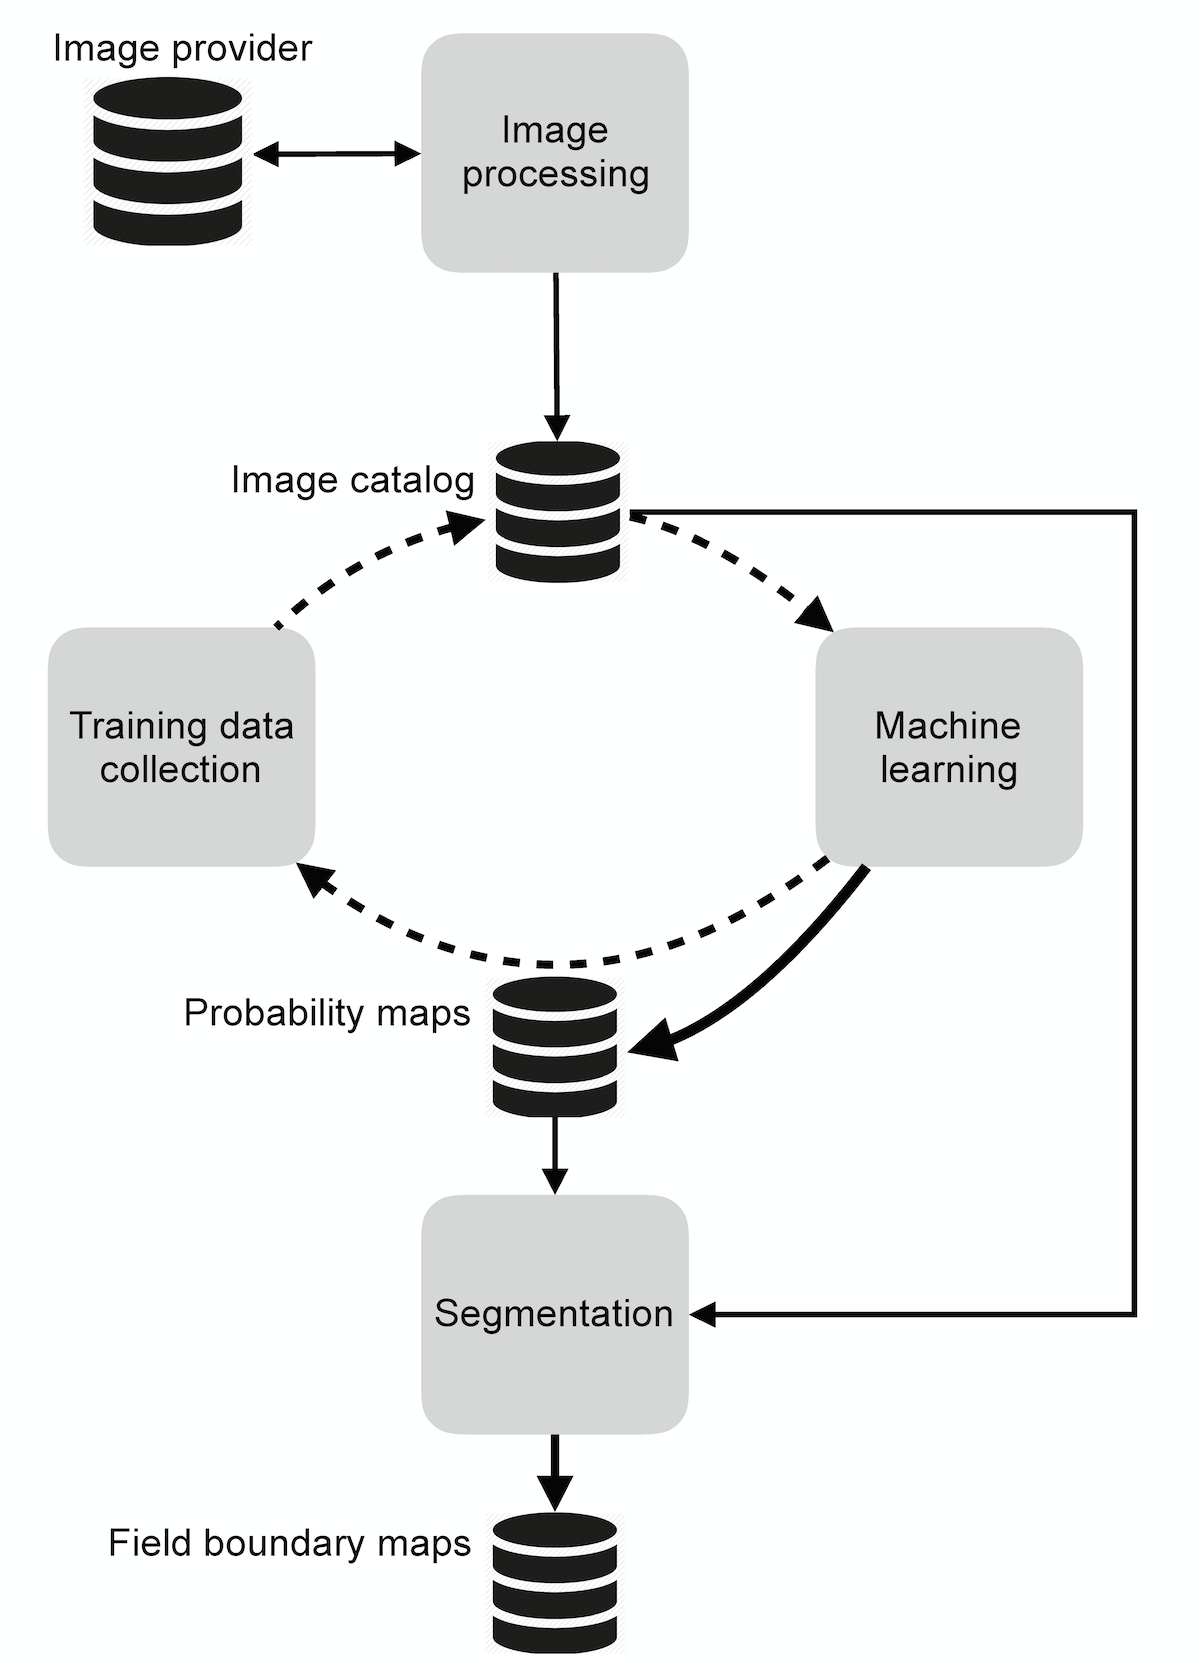
\includegraphics[width=0.5\linewidth]{figures/figure1} 

}

\caption{An overview of the primary mapping components, the data stores that hold the inputs and outputs from each component, and the direction of connections between them. The dashed line indicates iterative interactions, while solid lines indicate one-time or irregular connections.}\label{fig:systemoverview}
\end{figure}

We describe each component in further detail in the following section,
and how we applied them to map Ghana's annual cropland boundaries,
excluding tree crops.

\hypertarget{image-compositing}{%
\subsection{Image compositing}\label{image-compositing}}

The image processing component was designed for PlanetScope Analytic
surface reflectance imagery (PlanetTeam 2018), which provides three
visual (red, green, blue) and near-infrared bands at 3.7 m resolution at
nominal daily frequency. The images are provided as ortho-rectified and
converted to surface reflectance, although there are residual errors
from inter-sensor differences and the radiometric normalization process
(Houborg and McCabe 2018), variation in the orientation of scene
footprints, as well as a high frequency of cloud cover over the study
region (Wilson and Jetz 2016, Roy et al. 2021) that are not fully
captured by the provided cloud masks. To minimize the effect of these
residual errors, we developed a procedure for creating temporal
composites of the primary growing and non-growing seasons within a
single 12-month period. For Ghana, we defined the primary growing season
as May through September, followed by the off (or dry) season from
November or December through February. We chose these two seasons
because prior work shows that the contrast between them improves
cropland classifications (Debats et al. 2016), Furthermore, capturing
the seasons in this sequence during the same year helps minimize
differences caused by land change. The wide time intervals we used to
define each season were necessary for collecting a sufficient number of
images to make high quality composites, as Ghana's cloud cover renders
many scenes unusable and therefore unavailable in Planet's catalog, thus
the effective return interval can be substantially longer than 24 hours
during the cloudiest months (Roy et al. 2021).

We collected all available scenes intersecting Ghana and falling within
these two seasons during the 2018 agricultural year (defined here as
March, 2018-February, 2019) via the Planet API (PlanetTeam 2018), and
transferred these to cloud storage (Amazon Web Services {[}AWS{]} S3).
We then converted each scene into analysis ready data (Dwyer et al.
2018) by cropping each to the boundaries of a 0.05\(^\circ\) grid that
it intersected (see Figure S1 in Supplemental Information {[}SI{]}),
which provided the dimensions for making composited image tiles. We
chose this cell size for tiling because it is slightly narrower than the
short axis of a PlanetScope scene, which increases the number of
intersecting scenes that completely cover the tile, thereby helping to
minimize edge artifacts in the composites.

To create a seasonal composite, we calculated two weights for the time
series of each pixel within the ARD stack for a given season:

\begin{equation} \label{eq:cloud}
\mathrm{W1_t} = \frac{1}{\mathrm{blue_t}^2}
\end{equation}

\begin{equation} \label{eq:shadow}  
\mathrm{W2_t} =\begin{cases}
    \frac{1}{\mathrm{NIR_t}^4}, & \text{if $\mathrm{NIR_t}$ < median\{$\mathrm{NIR_{t1}}$, $\mathrm{NIR_{t2}}$, ..., $\mathrm{NIR_{ti}}$\}}.\\
    1, & \text{otherwise}.
  \end{cases}
\end{equation}

Where \emph{t} is a particular date in the pixel time series, which
begins at date 1 for the given compositing period and ends on date
\emph{i}, \emph{blue} is the blue band, and \emph{NIR} the near infrared
band. Equation \ref{eq:cloud} assigns lower weights to hazy and clouded
pixels as the blue band is sensitive to these atmospheric features
(Zhang et al. 2002), while Equation \ref{eq:shadow} assigns low weights
to pixels in cloud shadow (Zhu and Woodcock 2012, Qiu et al. 2020)

After assigning these two weights, we calculated the final composited
pixel value:

\begin{equation}
\mathrm{\bar{B} = \frac{\sum_{t=1}^{T}B_t * W1_t * W2_t}{\sum_{t=1}^{T}W1_t * W2_t}}
\end{equation}

Which is the weighted mean for each pixel for each band \emph{B} for the
given season.

Each composited seasonal tile was saved as a cloud-optimized geotiff,
and a ``slippy
map\footnote{https://wiki.openstreetmap.org/wiki/Slippy\_Map}''
rendering was created for each composite using Raster Foundry (Azavea
2020), for display within the labelling platform (next section).

We generated a catalog of 16232 composite tiles (hereafter simply
``tiles'') for Ghana, consisting of a seasonal pair for each of the 8116
0.05\(^\circ\) tile grid cells covering Ghana. To assess the quality of
the resulting composites, 50 tile grid cells were randomly selected, and
two separate observers graded each corresponding seasonal composite
using a four category that evaluated the degree of 1) residual cloud and
2) cloud shadow, 3) the number of visible scene boundary artifacts, and
4) the proportion of the image with resolution degraded below the 3.7 m
PlanetScope resolution (e.g.~because of between-date image
mis-registrations). Each category was qualitatively ranked from 0-3,
with 0 being the lowest quality, and 3 the highest (see SI for complete
protocol), making the highest possible score 12. We rescaled scores to
fall between 0 and 1.

\hypertarget{mapping-cropland-probabilities-with-active-learning}{%
\subsection{Mapping cropland probabilities with active
learning}\label{mapping-cropland-probabilities-with-active-learning}}

The first step in creating a country-wide field boundary map of Ghana
was to create a pixel-wise classification of cropland probabilities
throughout the country. Given the high resolution of the imagery and the
need to minimize the computational burden, we divided Ghana into 16
distinct mapping regions, or Areas of Interest (AOIs). We constructed
the AOIs by grouping together tile grids into blocks representing the
larger 1\(^\circ\) cells used to assign tile identifiers (Figure S1A).
We grouped tile cells from 1\(^\circ\) degree cells that overlapped
Ghana's boundaries together with those from the nearest 1\(^\circ\) cell
contained entirely within Ghana (with the exception of AOI 16, which was
comprised of tile grids from the 1\(^\circ\) cells along Ghana's
southern coast. The average extent of the resulting AOIs was 15,457
km\(^2\) (range 12,160-23,535 km\(^2\)).

We used the active learning process to develop a separate cropland
classification model for each of these AOIs, based on an approach
described by Debats et al (2017). We initiated the process by training a
starter model using labels from a set of randomly selected training
sites drawn from a 0.005\(^\circ\) grid that was nested within the
tiling grid. This finer grid, which we refer to as the ``primary grid''
for simplicity, provided the target area for creating labels (section
2.2.1), as well as the unit for distributing computing jobs (section
2.2.2). We then assessed the performance of the starter model against a
separate set of validation labels developed for each AOI, applied the
model to predict cropland probabilities for pixels in unlabelled primary
grid cells in each AOI, and calculated an uncertainty criterion (Debats
et al. 2017):

\begin{equation}
\mathrm{Q_I = \sum_{I(x, y) \epsilon I} (p(x, y) - 0.5)^2}
\end{equation}

Where Q is the uncertainty for each unlabelled primary grid cell I,
calculated from the predicted probability \emph{p} of a randomly
selected subset of pixels (x, y) drawn from it. Pixels with predicted
probabilities closer to 0.5 are least certain as to their
classification, thus the lowest values of \(Q\) represent primary grid
cells posing the most difficulty for the classifier.

We ranked the unlabelled primary grid cells from least to most certain,
randomly selected a subset of cells from the top 30\% of the ranking (to
minimize the risk of spatial autocorrelation), and sent these back to
the labelling platform. After these new sites were labelled, they were
added to the starter pool of labels, the model was retrained with the
larger training set, its performance and prediction uncertainty was
reassessed, and a new sample of the most uncertain primary grid cells
was again sent for labelling. This loop repeated until model performance
gains saturated or reached a pre-defined threshold, after which a final
map of cropland probabilities was made for the AOI.

In the next two sections, we describe the labelling and machine learning
components of the active learning process in more detail.

\hypertarget{labelling}{%
\subsubsection{Labelling}\label{labelling}}

To collect the initial randomized samples for model training, we grouped
the AOIs (Figure S1A) into three clusters based on approximate
agro-ecological similarity: the 6 northernmost savanna-zone AOIs
(Cluster 1), a central to southeastern cluster (Cluster 2) consisting of
the 3 middle (AOIs 7-9) and 2 southeastern AOIs (12 and 15), and a
southwestern cluster (Cluster 3) made up of the forest zone AOIs (10,
11, 13, 14, 16). Within each cluster, we randomly selected and labelled
500 primary grid cells, which provided relatively large initial training
samples for these agro-ecologically similar regions, while helping to
minimize the overall amount of labelling effort. To create validation
samples, we randomly selected and labelled 100 primary grid cells per
AOI, and a further 100 cells were labelled in each AOI during each
active learning iteration.

In addition to training and validation labels, we also collected
training reference labels and map reference labels (Elmes et al. 2020).
The former were a set of 98 primary grid cells selected to represent the
range of cropland types and densities in Ghana, which were labelled by
expert analysts (the lead researchers on this project). We used these to
assess the performance of the individual labellers collecting training
and validation labels. Map reference labels were collected and used to
assess the accuracy of the final map (see Section 2.4).

We collected all labels using a custom-built platform that we adapted
from an earlier prototype we developed for crowdsourced labelling (Estes
et al. 2016a). We enhanced this platform by making several major
additions, including an independent backend that allowed us to recruit
and manage our own labelling teams, improved procedures for assessing
and improving label accuracy, and processes for automating the machine
learning component. The platform runs on a cloud-hosted Linux virtual
server (AWS EC2) and is comprised of a database (PostGIS/Postgres), a
mapping interface (OpenLayers 3), an image server (Raster Foundry), and
a set of utilities for managing, assessing, and converting digitized
field boundaries into rasterized labels.

We created a separate labelling instance for each AOI. To create
training and validation labels, labellers (the co-authors of this paper)
logged into the website (built with Flask) for a particular AOI and
navigated to the mapping interface (Figure \ref{fig:labeller}), where
they were presented with a white target box representing a primary grid
cell to label, a set of digitizing tools, and several different sources
of imagery. These included true and false color renderings of the
growing season and dry season PlanetScope composites, and several
virtual globe basemaps. They then used the polygon drawing tool to
digitize the boundaries of all crop fields visible within the
PlanetScope overlays that intersect the target grid cell. For this
project, labellers were instructed to digitize active or recently active
crop fields, avoiding tree crops, and fallow or potentially abandoned
fields (see SI for digitizing rules) To aid with interpretation,
labellers toggled between the PlanetScope renderings and the basemaps to
help form a judgement about what constitutes a field. The labeller
assigned each digitized polygon a class category (e.g.~annual cropland),
saved all completed fields to the database, and were then presented with
the next target to label. If the target grid cell did not contain any
fields, labellers simply pressed save to go to the next cell.

\begin{figure}

{\centering 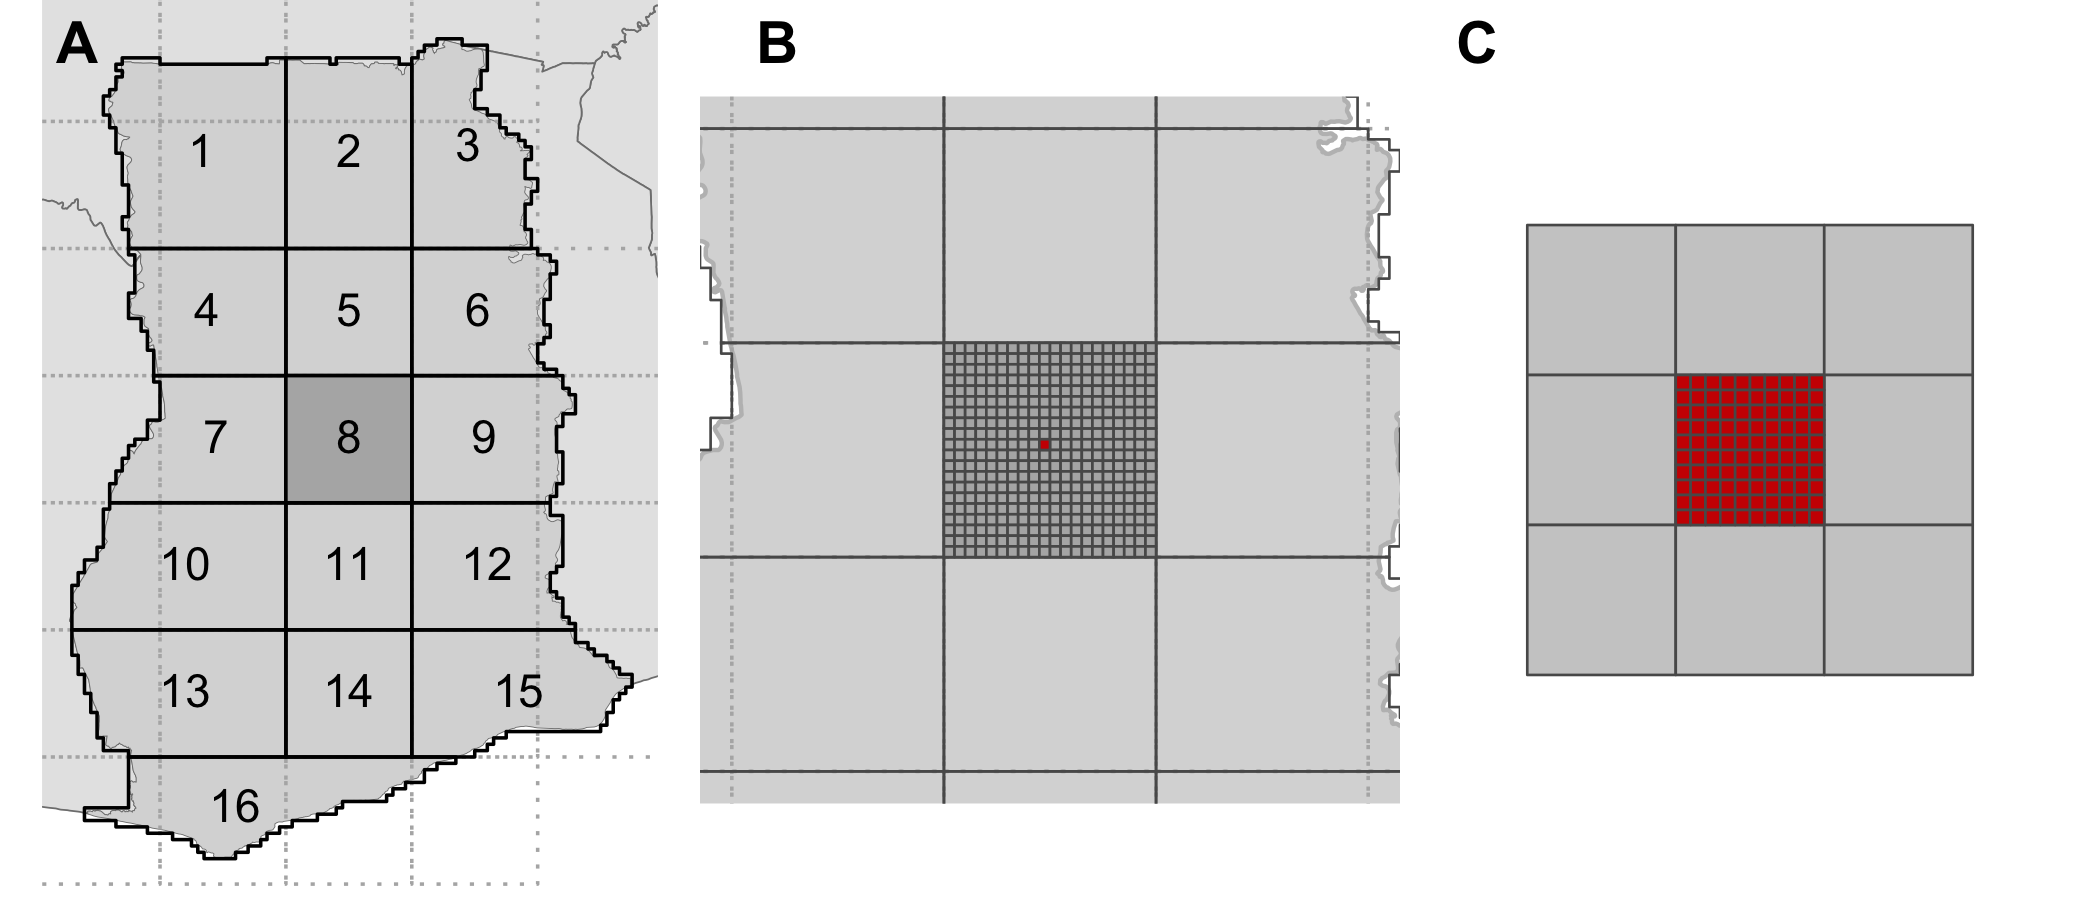
\includegraphics[width=0.95\linewidth]{figures/figure2} 

}

\caption{An overview of the labelling platform's interface}\label{fig:labeller}
\end{figure}

The flow of labelling targets presented to each worker was determined by
the platform's built-in scheduler. Each primary grid cell selected for
labeling was placed into a queue within the platform's database, and
converted into a labelling \emph{task} with a specified number of
\emph{assignments} (the boundaries drawn by an individual labeller) that
had to be completed in order to finish the task. There were two types of
tasks, accuracy assessment or model training/validation, with the
assignments for each indistinguishable to labellers. Upon completing an
accuracy assessment assignment, the platform invoked a scoring algorithm
that compared the labeller's digitized boundaries against a set of
training reference polygons, resulting in a label quality score:

\begin{equation} \label{eq:qaqc}
\mathrm{score_i}=\beta_0\mathrm{I}+\beta_1\mathrm{O}+\beta_2\mathrm{F}+\beta_3\mathrm{E}+\beta_4\mathrm{C}
\end{equation}

Where \emph{i} indicates the particular assignment, and \(\beta_{0-4}\)
represent varying weights that sum to 1. \emph{I} refers to ``inside the
box'' accuracy, \emph{O} is the accuracy of those portions of the
labeller's polygons extending beyond the target grid boundaries,
\emph{F} is fragmentation accuracy, a measure of how many individual
polygons the labeller delineated relative to the reference, \emph{E}
measures how closely each polygon's boundary matched its corresponding
reference polygon boundary, and \emph{C} assesses the accuracy of the
labeller's thematic labels (see SI for individual formulae). Equation
\ref{eq:qaqc} is an extension of the approach described by Estes et
al.~(2016).

We configured the platform's scheduler to present workers with accuracy
assessment assignments at a rate of 1 for every 5 assignments mapped.
This generated a history of accuracy assessment scores that we used to
assess label quality and minimize label error.

For training and validation, where there was no reference data to assess
label accuracy, we set each task to have four assignments, i.e.~each was
completed by four separate labellers. When all four assignments were
complete, a Bayesian merging routine was invoked to combine the four
sets of labels into a single consensus label:

\begin{equation}
P(\theta|\mathrm{D})=\sum_{i=1}^{n}\mathrm{P}(\mathrm{W_i}|\mathrm{D})\mathrm{P}(\mathrm{\theta}|\mathrm{D}, \mathrm{W_i})
\end{equation}

Where \(\theta\) represents the true cover type of a pixel (field or not
field), \emph{D} is the label assigned to that pixel by a labeller, and
\(W_i\) is an individual labeller. P(\(\theta\)\textbar D) is the
probability that the actual cover type is what the labellers who mapped
it says it is, while P(W\(_i\)\textbar D) is the average score (ranging
between 0 and 1) of the accuracy assessment assignments an individual
labeller completed within the AOI, and P(W\(\theta\)\textbar D,
\emph{W}\(_i\)) is the labeller's label for that pixel. This approach
therefore used the average assignment quality score for to weight each
labeller's label for a given pixel (see SI for further details). Each
pixel in the target grid cell was merged using this approach (n =
40000), which helps to minimize individual labellers' errors. We
estimated a confidence measure for each consensus label by calculating
its Bayesian Risk (see SI), which ranges between 0 and 1, with 0
indicating full agreement between labellers for all pixels, and 1
indicating complete disagreement.

\hypertarget{cropland-classification-model}{%
\subsubsection{Cropland classification
model}\label{cropland-classification-model}}

Upon completing each batch of labels, the platform automatically
launched a machine learning cluster (Elastic Map
Reduce\footnote{https://docs.aws.amazon.com/emr/latest/APIReference/emr-api.pdf})
comprised of several hundred to a thousand CPUs, depending on the size
of the AOI.

The first step in the process was to derive a set of features from the
image composites. Previous work showed that a large number of simple
features summarizing image reflectance and vegetation indices within
local neighborhoods were highly effective for classifying smallholder
croplands (Debats et al. 2016). We followed that logic in this study,
but used a smaller feature set because the storage and memory required
for our mapping geographies were several orders of magnitude larger. For
each seasonal composite, we calculated the mean and standard deviation
of each band within an 11X11 and 5X5 moving window, respectively
(initial tests revealed these two window sizes to be most effective).
This provided an overall set of 24 features, including the unmodified
bands of both composites (Table 1).

\begin{center}Table 1. List of image features.\end{center}

\begin{longtable}[]{@{}lll@{}}
\toprule
Feature & Window Size & N Features \\
\midrule
\endhead
RGB-NIR & 1X1 & 8 \\
Mean & 11X11 & 8 \\
Standard deviation & 5X5 & 8 \\
\bottomrule
\end{longtable}

We used a combination of
\texttt{GeoTrellis}\footnote{https://github.com/locationtech/geotrellis},
\texttt{rasterio}\footnote{https://rasterio.readthedocs.io/en/latest/},
and \texttt{RasterFrames}\footnote{https://rasterframes.io/} to derive
the features on the fly (which was enabled by converting the composites
to Cloud-optimized Geotiffs\footnote{https://www.cogeo.org/}) and
convert them into Apache Spark DataFrames. The extracted features were
combined with their corresponding training and validation labels and
passed to the machine learning classifier, a \texttt{SparkMLlib}
implementation of Random Forests (Breiman 2001). We trained the model
with a balanced sample and a tree depth of 15 and total tree number of
60, which initial testing showed to provide a reasonable balance between
computational time and performance.

\hypertarget{model-performance}{%
\subsubsection{Model performance}\label{model-performance}}

To assess performance of the Random Forests classifier, we used the
validation sample to calculate binary accuracy, the F1 score (the
geometric mean of precision and recall), and the area under the curve of
the Receiver Operating Characteristic (Pontius and Si 2014), as well as
the false positive rate. We calculated these measures each time the
model was retrained for a given AOI, in order to assess the change in
classifier performance with each active learning iteration.

To evaluate whether active learning improved model performance relative
to randomized label selection, we ran an additional test within three
AOIs (1, 8, and 15), in which we retrained the model with 100 randomly
selected labels for each iteration. We then compared the differences in
accuracy, AUC, and F1 between the actively and randomly trained models
(Debats et al. 2017).

To quantify the potential impact of label error on classification
results, we conducted two further analyses. We evaluated the performance
differences between models trained with three different sets of labels:
1) those from the lowest scoring labeller to map each training site, 2)
those from the highest scoring labeller, and 3) the consensus labels. We
also calculated the correlations between the mean Bayesian Risk of
labels in each AOI and the corresponding model performance metrics
(Table S3).

\hypertarget{segmentation}{%
\subsection{Segmentation}\label{segmentation}}

Upon completion of the active learning process, we deployed a five-step
algorithm to create a segmented map of field boundaries. In the first
step, we identified edge features within the imagery. To do this, we
applied the meanshift algorithm (Yizong Cheng 1995) to each dry-season
composite tile, and then passed a Sobel filter over the mean-shifted
green, red, and near-infrared bands, and the corresponding map of
predicted cropland probabilities. We then summed the four resulting edge
images to produce a combined edge image.

In the second step, we used a compact watershed algorithm (Neubert and
Protzel 2014) to segment the edge image, specifying a high number of
segments (6,400) segments per tile, so that the mean segment size
(\textless0.5 ha) was finer than the expected mean field size
(\textgreater1 ha).

In the third step, we hierarchically merged the resulting polygons. We
first constructed a region adjacency graph for each tile, with each node
representing all image pixels within each polygon. The edge between two
adjacent regions (polygons) was calculated as the difference between the
means of the normalized colors of all bands. We then merged the most
similar pairs of adjacent nodes until there were no edges remaining
below the predetermined threshold of 0.05.

In the fourth step, we overlaid the merged polygons with the cropland
probability images, and polygons in which the mean probability was
greater than 0.5 were retained as crop fields.

In the fifth and final step, we refined the crop field polygons, by
removing holes and smoothing boundaries using the Visvalingam algorithm
(Visvalingam and Whyatt 1993). We then merged neighboring polygons that
overlapped along tile boundaries.

The resulting map represents dry season crop field boundaries, as we did
not segment growing season images. We made this choice because labels
were primarily drawn on dry season composites, when boundaries were
typically more visible.

\hypertarget{map-assessment}{%
\subsection{Map assessment}\label{map-assessment}}

We followed recommended guidelines (Stehman and Foody 2019) to conduct
an independent assessment of the categorical accuracy of the final maps,
using a set of 1207 (487 cropland; 720 non-cropland) point-based, map
reference labels, which were placed across Ghana using a stratified
random sample design, and collected through the labelling platform by
two expert supervisors (see SI for full details on sample design and
collection). For efficiency, the supervisors labelled separate portions
of the sample, but overlapped on a small subset (n = 23). We calculated
the label agreement (87\%) on this subset to estimate uncertainty in the
map reference sample (Stehman and Foody 2019). In addition to this, the
sample was labelled with four classes: cropland; non-cropland; unsure
but likely cropland; unsure but likely non-cropland. The last two
classes, which constituted 15.7\% of the sample, provided a further
measure of uncertainty in the map reference sample

We used the sample to calculate the overall accuracy for each map, the
class-wise User's and Producer's accuracy, and the 95\% confidence
intervals for each accuracy measure (Olofsson et al. 2013, 2014, Stehman
and Foody 2019). We calculated these measures across the entire country,
as well as several different zones, to evaluate regional difference in
accuracy. We defined two sets of zonations (Figure S4), each containing
four zones, the first created by grouping 1) the three northern AOIs
(1-3), 2) the six central AOIs (4-9), 3) the four southwestern AOIs (10,
11, 13, 14, 16), and 4) the two southeastern zones (13, 15). This
grouping differs from the three clusters used to collect initial model
training samples, as we designed these to divide the country more
finely, and to isolate the less forested southeastern third of Ghana
from the more forest northwest. The second zonation was developed by
grouping the country's eight agro-ecological zones into four broader
clusters (Figure S4B). We applied this zonation only to the per-pixel
classification, to better understand patterns of error in the model.

To assess how effectively the segmentations captured field
characteristics, we compared the size class distributions of the
segmented field boundaries against the field boundaries digitized by the
labellers' over the 100 validation sites in each AOI. We chose this
approach because of existing uncertainties in polygon-based accuracy
assessment methods (Ye et al. 2018), and because the map's ability to
represent field sizes was of greatest interest. To undertake this
comparison, we selected the polygons from the most accurate labeller to
digitize the 100 validation grids in each AOI, and calculated the
average area and number of polygons in each cell. We then calculated the
same statistics from the segmented boundaries that intersected each
validation grid, and compared the two sets of statistics.

We used the final maps to evaluate the characteristics of Ghana's
croplands. We calculated the estimated area of cropland in Ghana, as
well as the average size and total number of fields in the different
AOIs. We used the map reference sample to calculate adjusted area
estimates and confidence intervals for each map class, and used the
differences between labellers' polygons and segmented boundaries at
validation sites to calculate bias-adjusted estimates of mean field
sizes and the total number of fields.

\hypertarget{results}{%
\section{Results}\label{results}}

Our results produced two separate maps of Ghana's annual croplands, over
a total area of 248,343 km\(^2\) that included portions of the
neighboring countries overlapped by image tiles.

\hypertarget{image-quality}{%
\subsection{Image quality}\label{image-quality}}

The assessment of image composites found that their quality in both
seasons was highest in the northern half of the country and lowest in
the southwest, (Figure \ref{fig:imqual}A), where the substantially
greater cloud cover resulted in a much lower density of available
PlanetScope imagery for each time period (Figure S5). The average
quality score of growing season composites was 0.88, with 70 percent
having scores \(\geq\) 0.85 (out of 1; Figure \ref{fig:imqual}B), while
the mean score of dry season composites was 0.92 (74 percent \(\geq\)
0.85).

\begin{figure}

{\centering 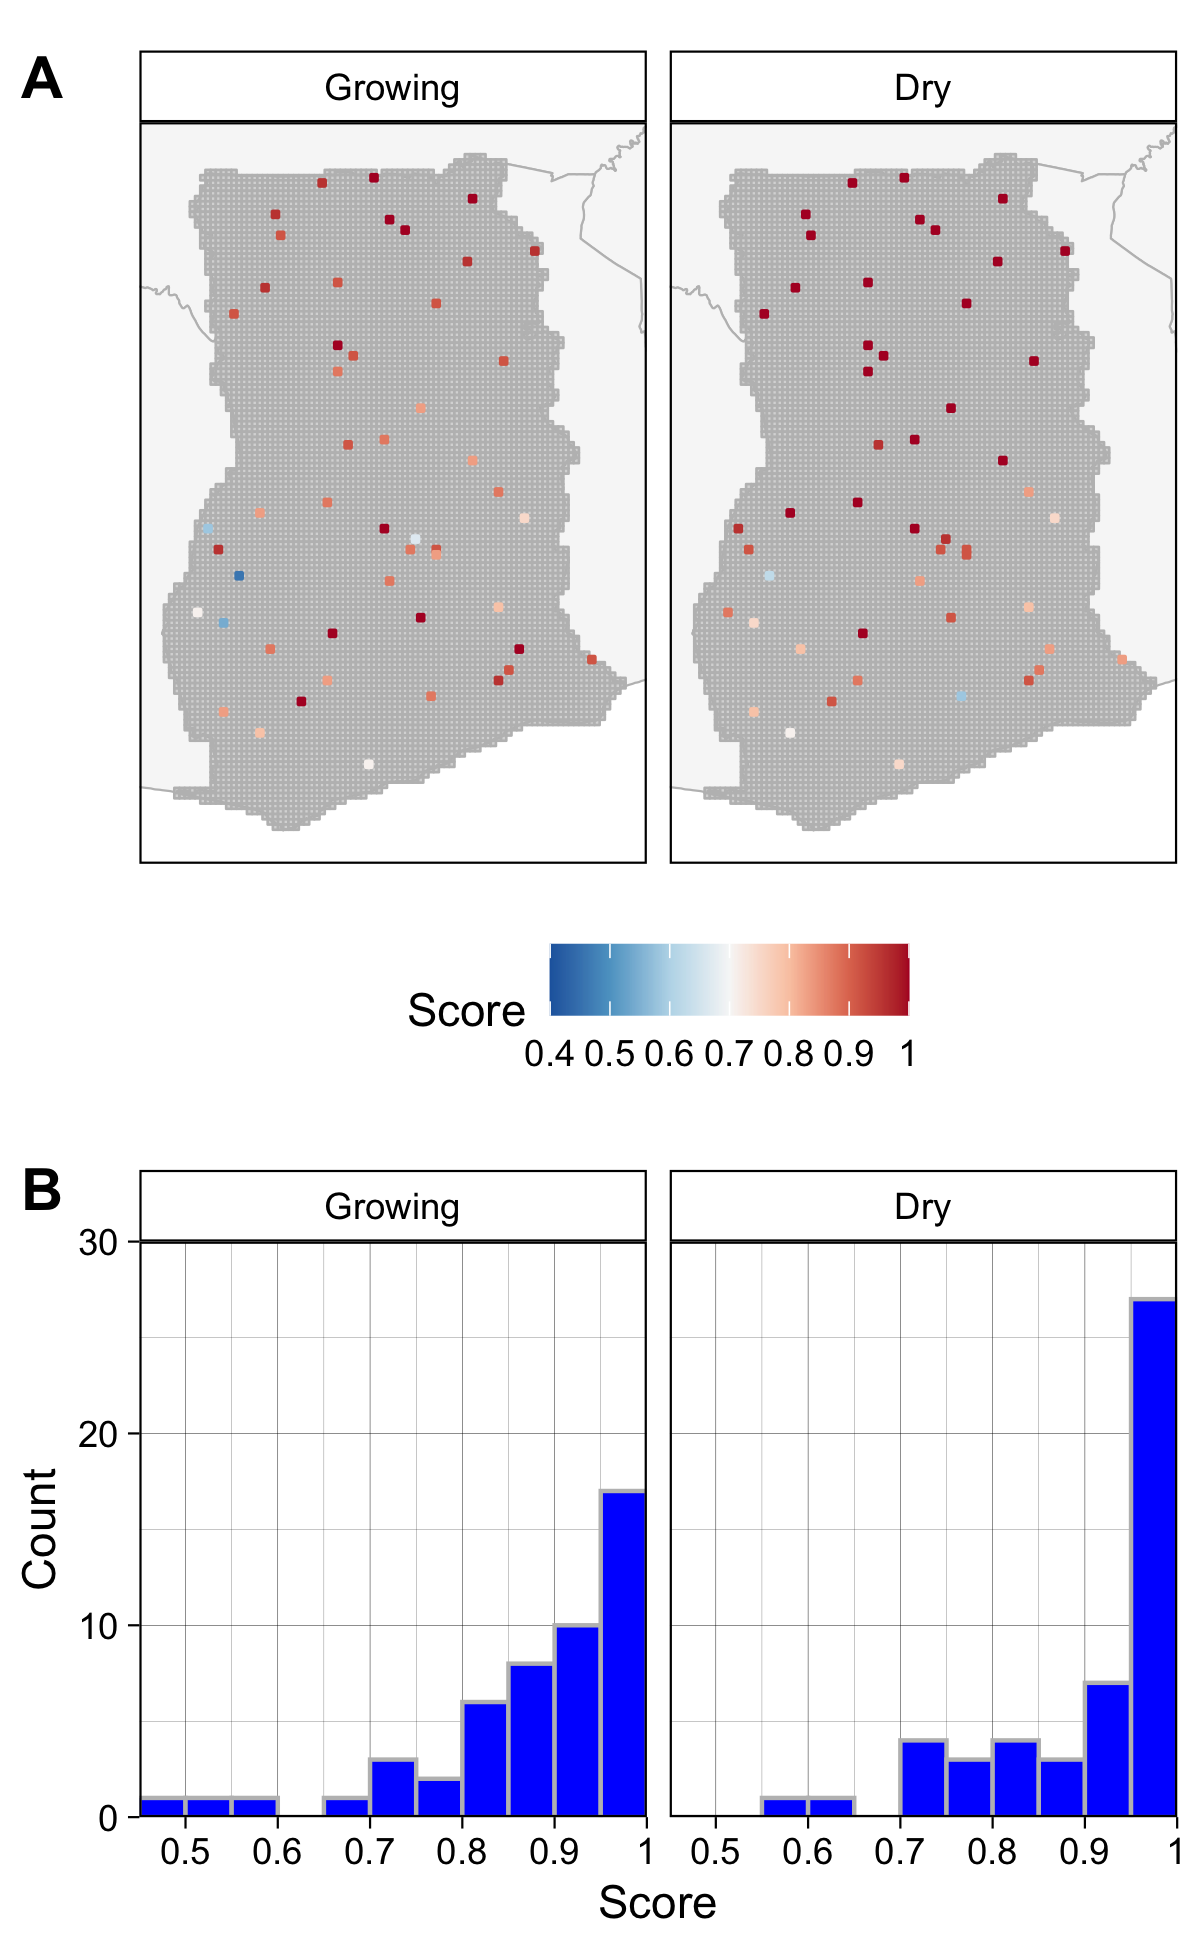
\includegraphics[width=0.7\linewidth]{figures/figure3} 

}

\caption{The location and quality scores of 100 randomly selected tiles for the growing (A) and off-growing season (B), and the corresponding distributions of the quality scores for each season, respectively (C and D).}\label{fig:imqual}
\end{figure}

\hypertarget{cropland-probabilities}{%
\subsection{Cropland probabilities}\label{cropland-probabilities}}

To make the initial maps of cropland probabilities, the active learning
process ran for 3 iterations in 12 of 16 AOIs, varying from as little as
1 to as many as 4 iterations across the other 4 AOIs, with the number of
iterations varying according to the performance of the starter models
(i.e.~AOIs with higher starting performance stopped after fewer
iterations, see SI). Each AOI's model was trained by 300-500 randomly
selected labels (Figure S6A), plus an additional 600 - 900 (typically
800) within each the AOI that were selected by active learning. Actively
selected labels showed distinctive patterns in several AOIs (Figure
S6B), such as concentrating along ecotones or the boundaries of
agro-ecological zones. A total of 6,299 training and 1,600 validation
labels were collected by 20 labellers to develop and assess model
performance (Figure S7).

\hypertarget{performance-gains-during-active-learning}{%
\subsubsection{Performance gains during active
learning}\label{performance-gains-during-active-learning}}

The performance of the Random Forest classifier typically improved with
each active learning iteration. The average accuracy, AUC, and F1 at
iteration 0 were 0.786, 0.809, and 0.464, respectively, increasing to
0.825, 0.818, and 0.507 by iteration 3 (Figure \ref{fig:alperformance}).
These differences represent respective gains of 4.9, 1.1, and 9.1
percent for the three metrics. The largest gains for each metric
occurred on iteration 1, averaging 2.9, 1, and 3.8 percent for accuracy,
AUC, and F1, while the lowest gains were realized on iteration 3, with
accuracy, F1, and AUC respectively increasing by just 1.2\%, 0.9\%, and
0.3\%. The scores achieved on the final iteration varied substantially
across AOIs and metrics. Accuracy ranged between 0.725 (AOI 15) and
0.948 (AOI 16), while AUC varied from 0.725 (AOI 4) and 0.93 (AOI 11),
and F1 from 0.252 (AOI 13) and 0.636 (AOI 8).

\begin{figure}

{\centering 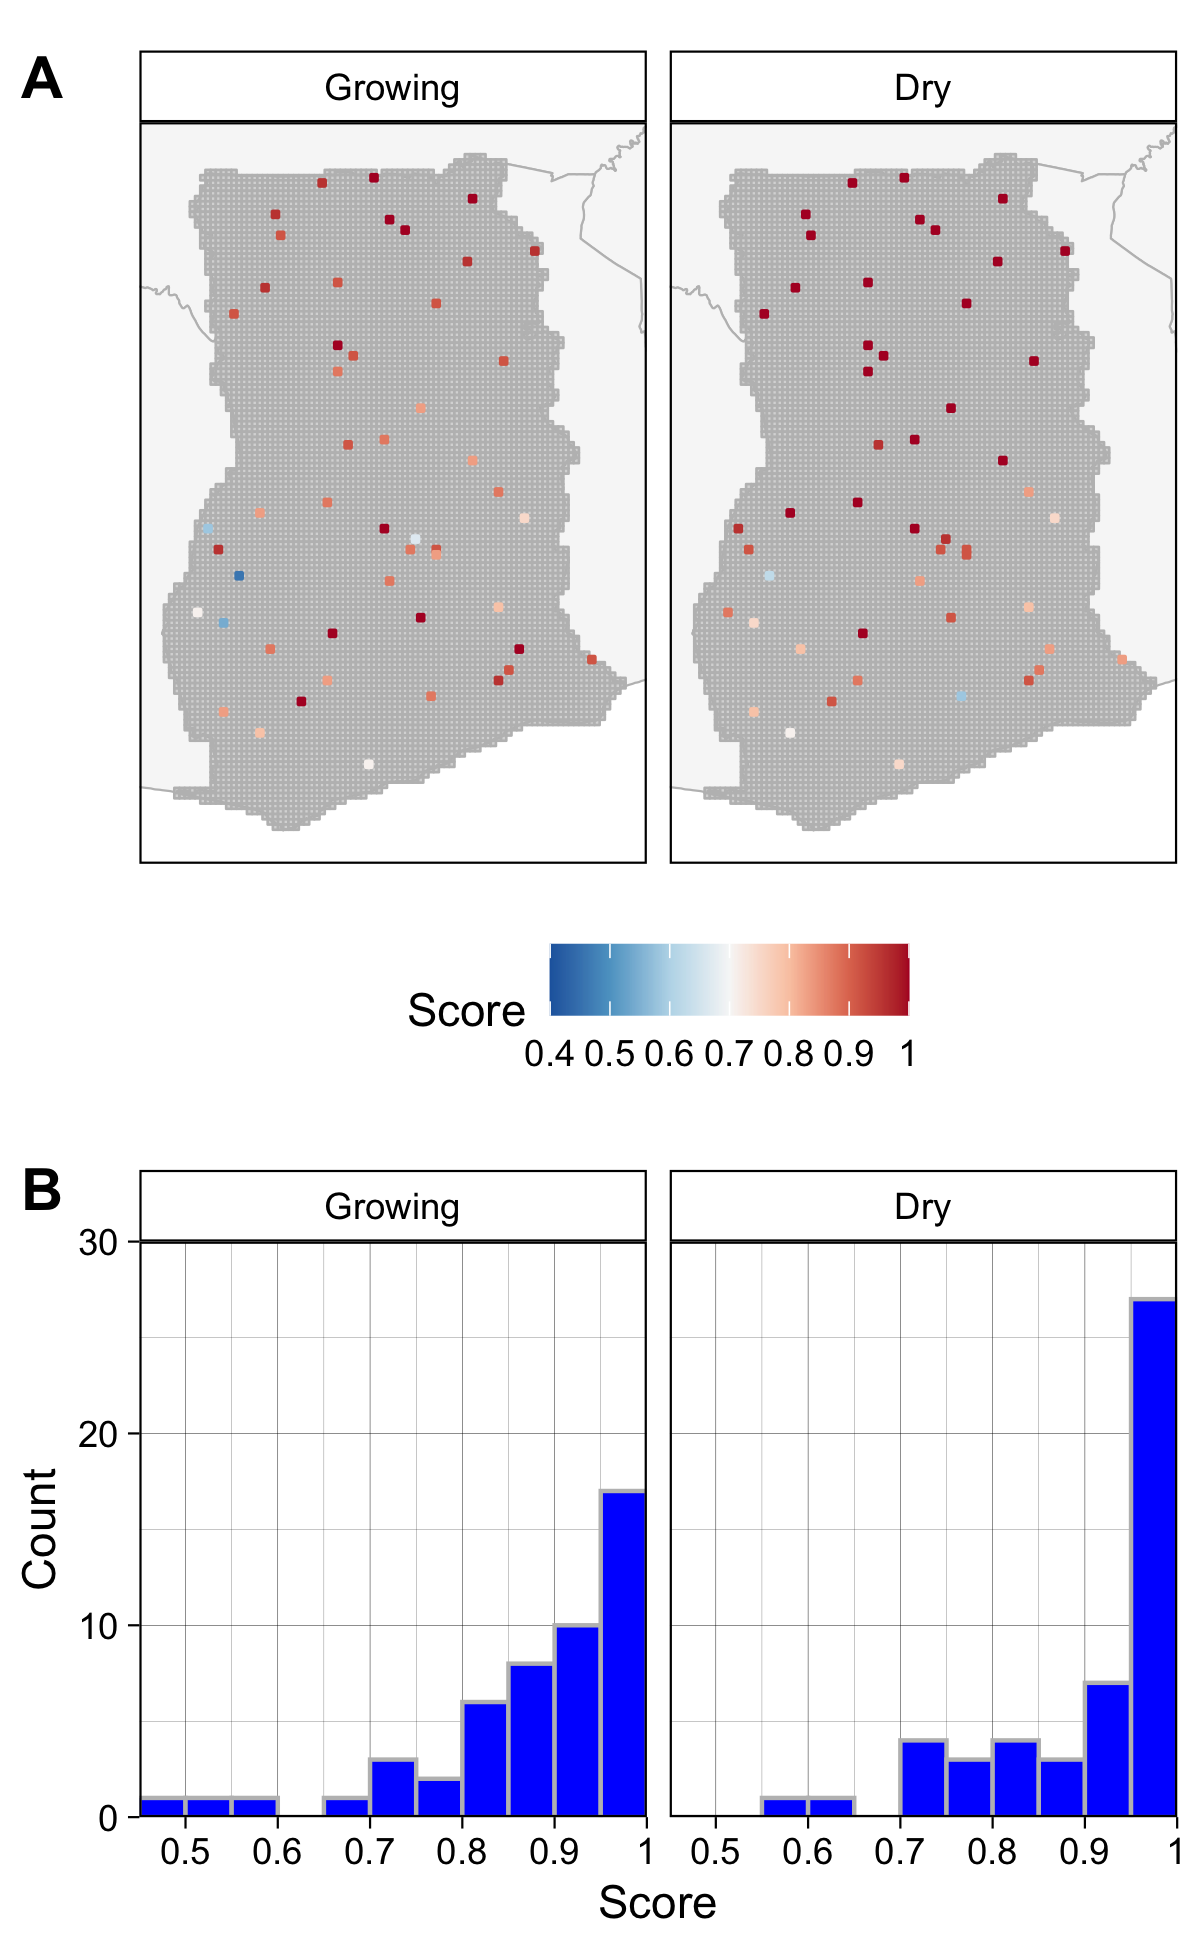
\includegraphics[width=1\linewidth]{figures/figure4} 

}

\caption{Scores for overall accuracy, area under the curve of the Receiver Operating Characteristic, and the F1 scores for the Random Forests model results after each iteration of the active learning loop for each AOI (gray lines), as well as the mean score per iteration across all AOIs (black lines).}\label{fig:alperformance}
\end{figure}

The experiment conducted in three AOIs (in AOIs 1, 8, and 15) showed
that training models with active learning improved performance compared
to randomized approaches to label selection. After three iterations, the
accuracy, AUC, and F1 scores for the actively trained models were
respectively 0.8, 0.6, and 2.3 percent higher than those for randomly
trained models (Figure S8). However, there was more variability in
earlier iterations, with average score differences of -1.7 (accuracy),
0.6 (AUC), and 0.8 percent (F1) after iteration 1, and -0.3 (accuracy),
0.4 (AUC), and 1.8 (F1) percent after iteration 2 (see SI for more
details).

\hypertarget{the-impact-of-label-error-and-uncertainty-on-model-performance}{%
\subsubsection{The impact of label error and uncertainty on model
performance}\label{the-impact-of-label-error-and-uncertainty-on-model-performance}}

We used the two measures of label quality calculated by the platform,
the average quality score of each labeller and Bayesian Risk (or simply
``label risk''), to assess the potential impacts of label error on model
performance. The average of each labeller's AOI-specific accuracy score
was 0.71 (range 0.6 to 0.85; see Figures S4 and S5 for details on label
scores and number of assignments per labeller). The average Bayesian
Risk was 0.124, with highest label risk (0.165) in the northern AOIs
(AOIs 1-6; Figures S6-7), lowest (0.165) in the southwestern AOIs (AOIs
10, 11, 13, 14, 16), and intermediate (0.131) in the
central-southeastern AOIs (AOIs 7-9, 12, 15).

Treating each labeller's average label quality scores (Figure S9) as a
proxy for error, we used these scores to develop training sets to test
the impact of label error on model performance. The results of these
tests, which were conducted in AOIs 1, 2, 8, and 15, showed that the
average accuracy, AUC, and F1 scores for models trained with the
consensus labels were respectively 0.772, 0.8, and 0.555 (Figure
\ref{fig:trainingimpact}). Performance metrics from consensus-trained
models were just 0.5 - 1.2 percent higher than those models trained with
the most accurate individuals' labels (accuracy = 0.762; AUC = 0.796; F1
= 0.55), but were 11.6 - 27.4 higher than models trained with the least
accurate individual labels (accuracy = 0.606; AUC = 0.716; F1 = 0.44).

\begin{figure}

{\centering 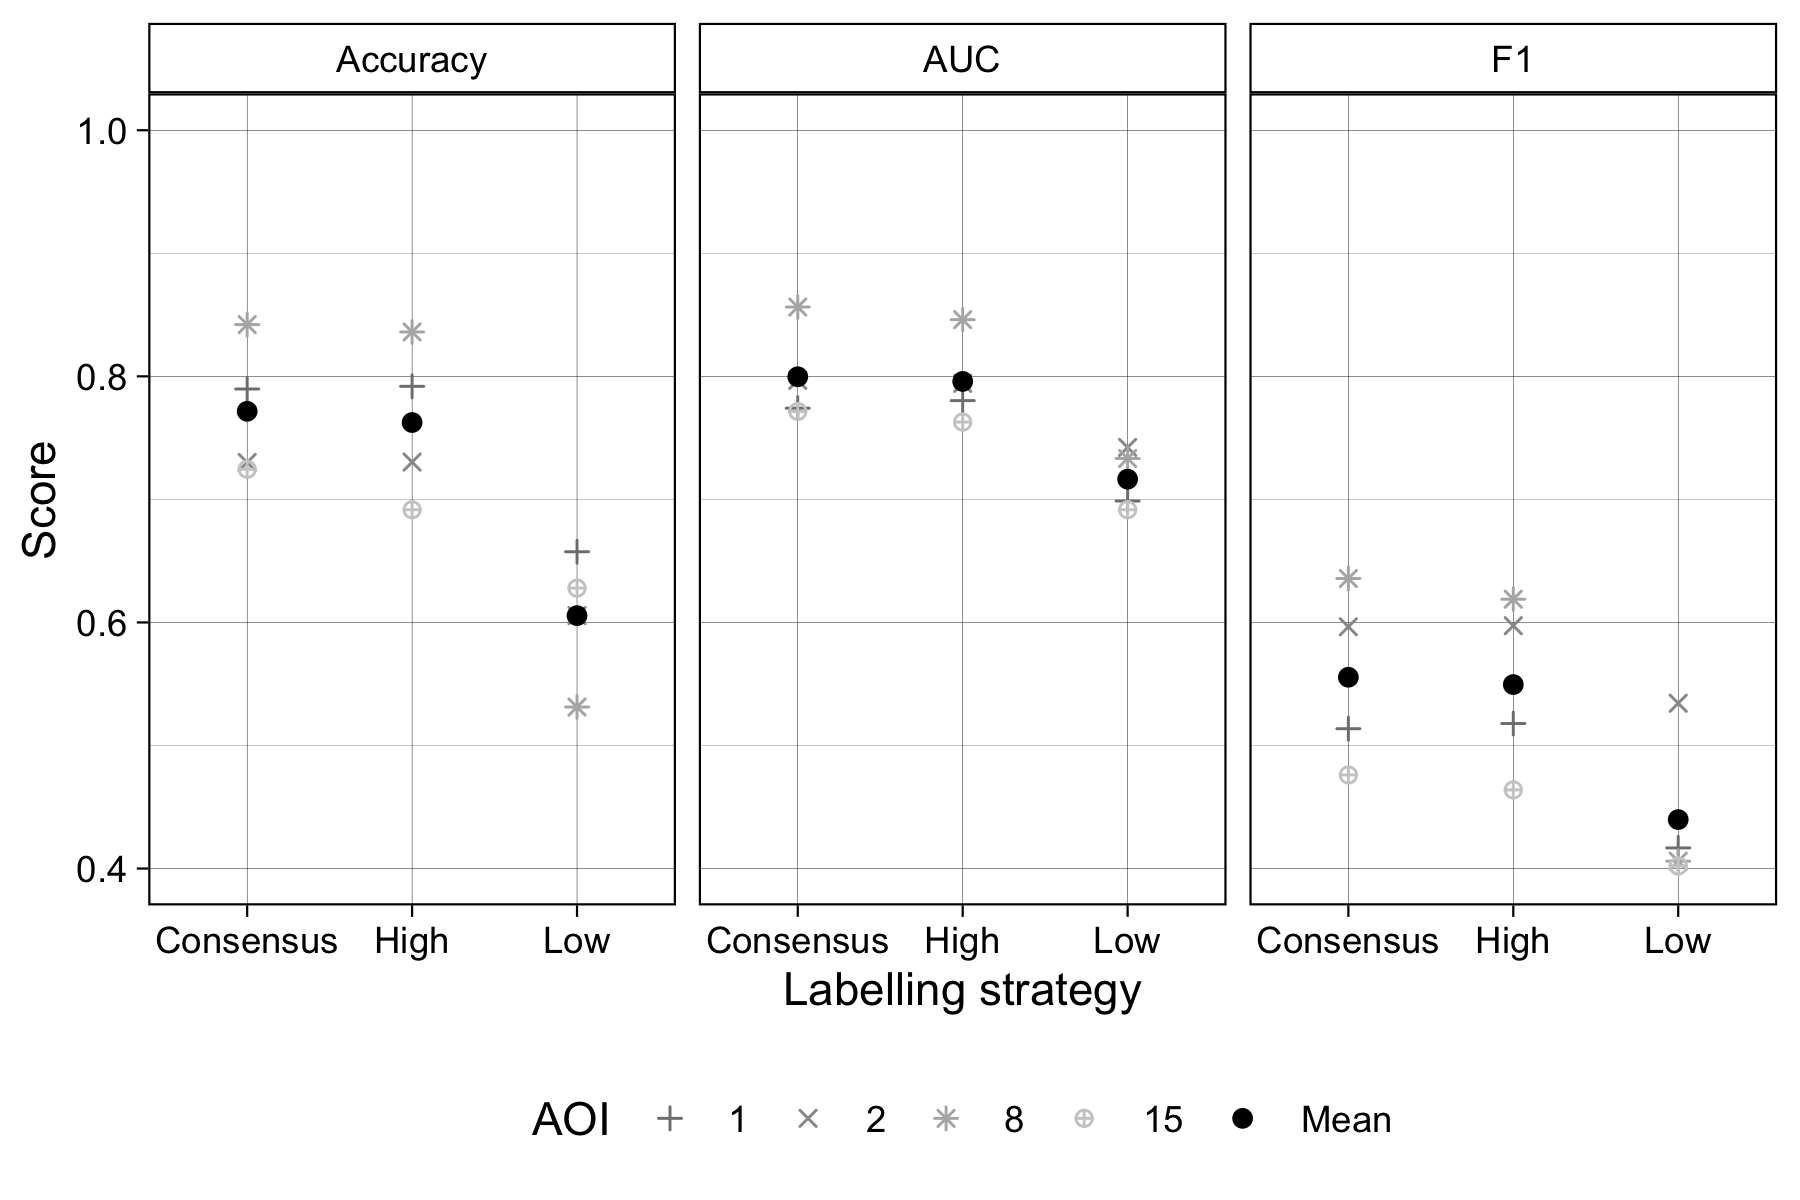
\includegraphics[width=1\linewidth]{figures/figure5} 

}

\caption{Scores for overall accuracy, area under the curve of the Receiver Operating Characteristic, and the F1 score resulting from models trained with consensus labels, and labels made by the most and least accurate labellers to map each site. Comparisons were made for AOIs 1, 2, 8, and 15, denoted by grey symbols, while the mean scores across these AOIs are shown for each metric.}\label{fig:trainingimpact}
\end{figure}

Correlations (Table S3) between the mean label risk per AOI (Figures
S10-11) and model performance metrics showed strong (Spearman's Rank
Correlation = -0.824) to moderate (r = -0.568) negative correlations
between label risk and accuracy and AUC, respectively, while F1 had a
weaker but moderate positive association (r = 0.456). The positive sign
of the latter relationship is counter-intuitive, but is explained by
risk's association with precision, one of two inputs to F1, which was
moderately positive (r = 0.629), whereas risk had a negligible
correlation with recall (r = 0.206), F1's other component. The
correlation between risk and the false positive rate (r = 0.688),
another important performance metric, shows that labelling uncertainty
may increase model commission error.

\hypertarget{map-accuracy}{%
\subsection{Map accuracy}\label{map-accuracy}}

\hypertarget{categorical-accuracy}{%
\subsubsection{Categorical accuracy}\label{categorical-accuracy}}

We used the map reference sample to evaluate the accuracy of the
cropland probability map (after classifying it using a threshold
probability of 0.5) and the map of segmented field boundary maps. We
found that the overall accuracy of the pixel-wise classifications was
88\% against this map reference sample (Table \ref{tab:mapaccuracy}).
Confining the map reference sample to four distinct zones (Figure S4A)
shows that overall accuracy ranged from 83.3\% in Zone 1 (AOIs 1-3) to
93.6\% in Zone 3 (AOIs 10, 11, 13, 15, and 16). The Producer's accuracy
of the cropland class was 61.7\% across Ghana, ranging from 45.6\% in
Zone 3 to 67.9\% in Zone 1, while the User's accuracy was 67.3\%
overall, ranging from 59.8\% in Zone 4 to 71.2\% in Zone 1. Both
measures of accuracy were substantially higher for the non-cropland
class across all zones, typically exceeding 90\%. The lowest accuracies
for the non-cropland class was in Zone 1 (Producer's = 89.3\%; User's =
87.7\%).

The overall accuracies obtained from the segmented maps were generally
1-2 percentage points lower than those of the per-pixel maps, while
User's accuracies tended to be 8-10 percentage points less (Table
\ref{tab:mapaccuracy}). In contrast, Producer's accuracies were 15-20
points higher than in the per-pixel map. The segmentation step therefore
helped to reduce omission error while substantially increasing
commission error.

\begin{table}
\caption{Map accuracies and adjusted area estimates for the ~3 m pixel-wise classifications (based on Random Forests predictions; top 5 rows) and the segmented map (bottom 5 rows). Results are provided for 4 zones (Zone 1 = AOIs 1-3; Zone 2 = AOIs 4-9; Zone 3 = AOIs 10, 11, 13, 14, 16; Zone 4 = AOIs 12, 15) plus the entire country. The error matrix (with reference values in columns) provides the areal percentage for each cell, and the Producer's (P), User's (U), and overall (O) map accuracies and their margins of error (in parenthesis) are provided, as well as the sample-adjusted area estimates (in km$^{2}$) and margins of error. }
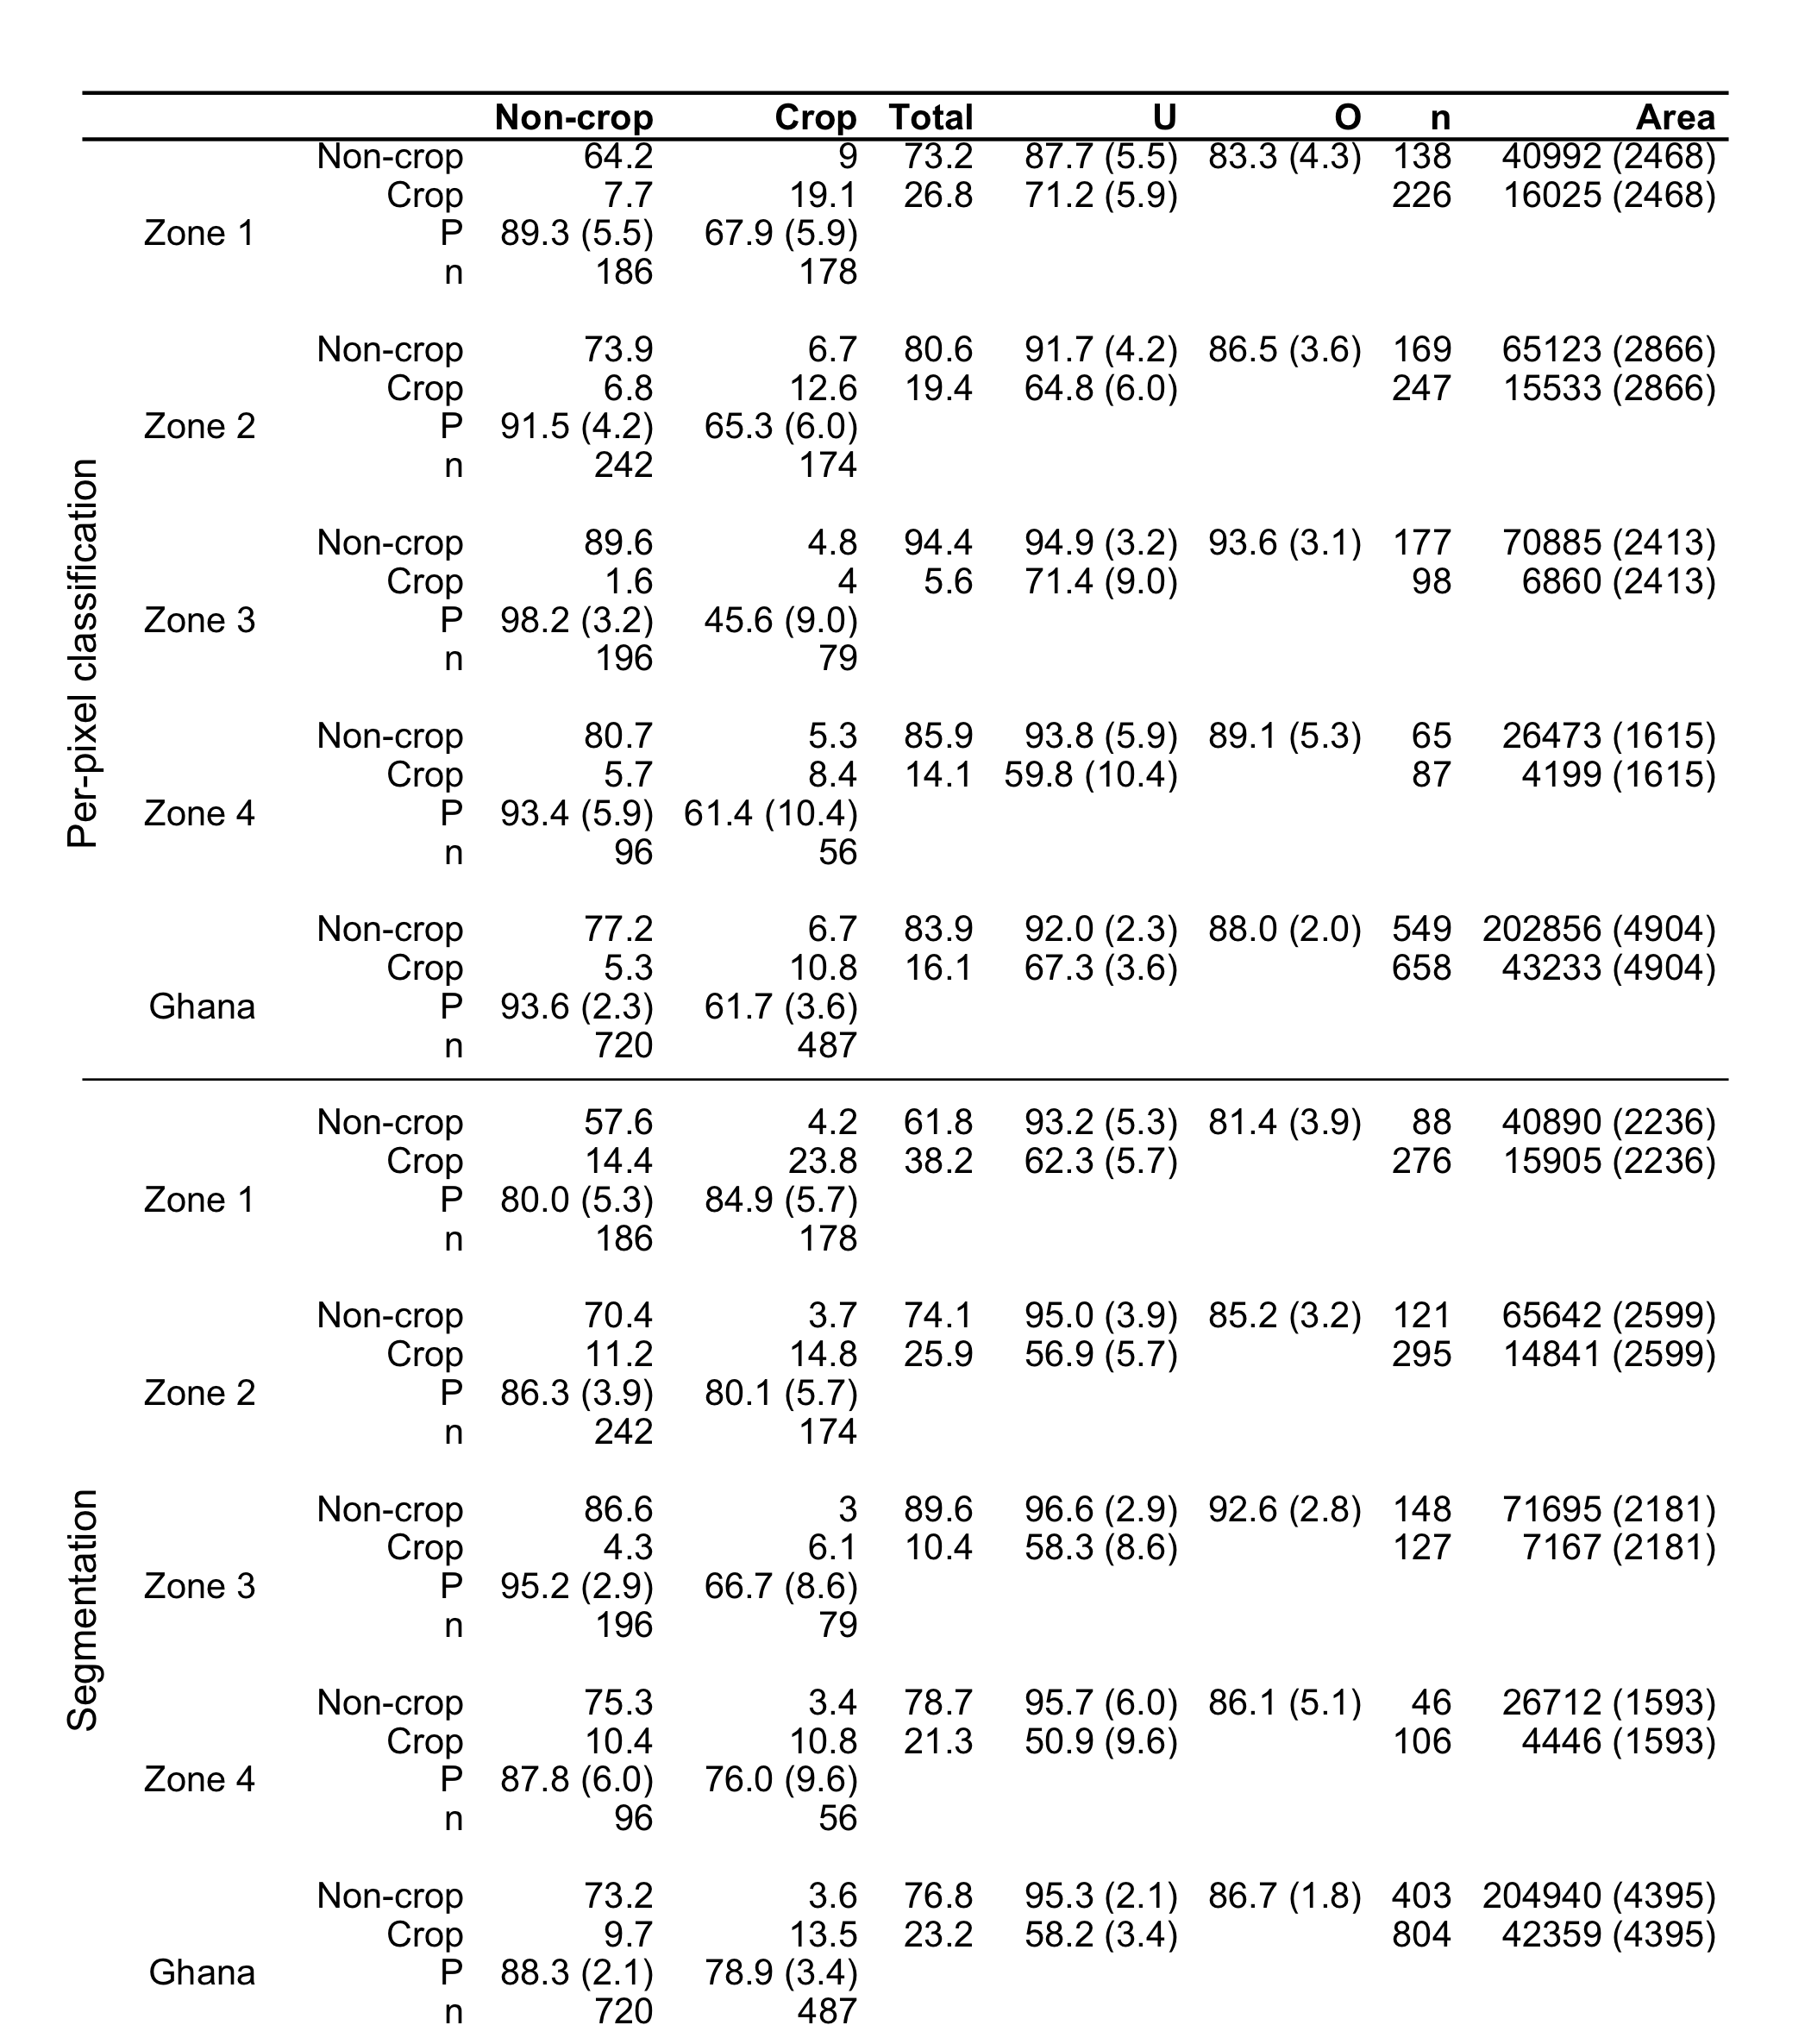
\includegraphics[width = 18cm]{figures/table2.png}
\label{tab:mapaccuracy}
\end{table}

\hypertarget{segmentation-quality}{%
\subsubsection{Segmentation quality}\label{segmentation-quality}}

The comparisons of digitized versus segmented field boundaries showed
that the mean field size across all validation sites averaged 4.97 ha
(Median = 3.75; StDev = 6.04), which was 1.41 times larger than the 2.06
ha (Median = 1.35; StDev = 3.26) mean area of labeller-digitized
polygons. This discrepancy was primarily caused by results in four AOIs
(2, 3, 7, and 15; Figure S13), where segments averaged between 7.76 and
10.76 ha, compared to 2.18 - 2.77 ha for the corresponding
hand-digitized polygons. The number of segmented fields per validation
site averaged 3.08 (median = 2.66; StDev = 2.9) compared to 4.4 (median
= 3.38; StDev = 4.52) for digitized polygons (Figure S14).

\hypertarget{ghanas-croplands}{%
\subsection{Ghana's croplands}\label{ghanas-croplands}}

Two separate maps of cropland were produced for each AOI, a per-pixel
map derived from the cropland probabilities, and the vectorized map of
field boundaries (Figure \ref{fig:mainmap}). The former provides the
more accurate picture of cropland distributions in Ghana, which are most
concentrated in the Southeastern corner (AOI 15), the central-western
region (AOI 7, the northeastern and northwestern corners of AOIs 10 and
11, and the south of AOI 8), and the northeastern quadrant stretching
from AOI 9 through AOIs 5 and 6 and up to AOIs 2 and 3. The northern
third of AOI 1 also has noticeable densities of cropland. Several
prominent areas of low cropland density indicate the presence of large
protected areas, such as Mole National Park in the southeastern corner
of AOI 1 and Digya National Park in the northwestern corner of AOI 12.
The relative absence of cropland in AOIs 13, 14, and 16 does not reflect
the scarcity of agriculture in these areas, but rather the predominance
of tree crops, which we did not map.

\begin{figure}

{\centering 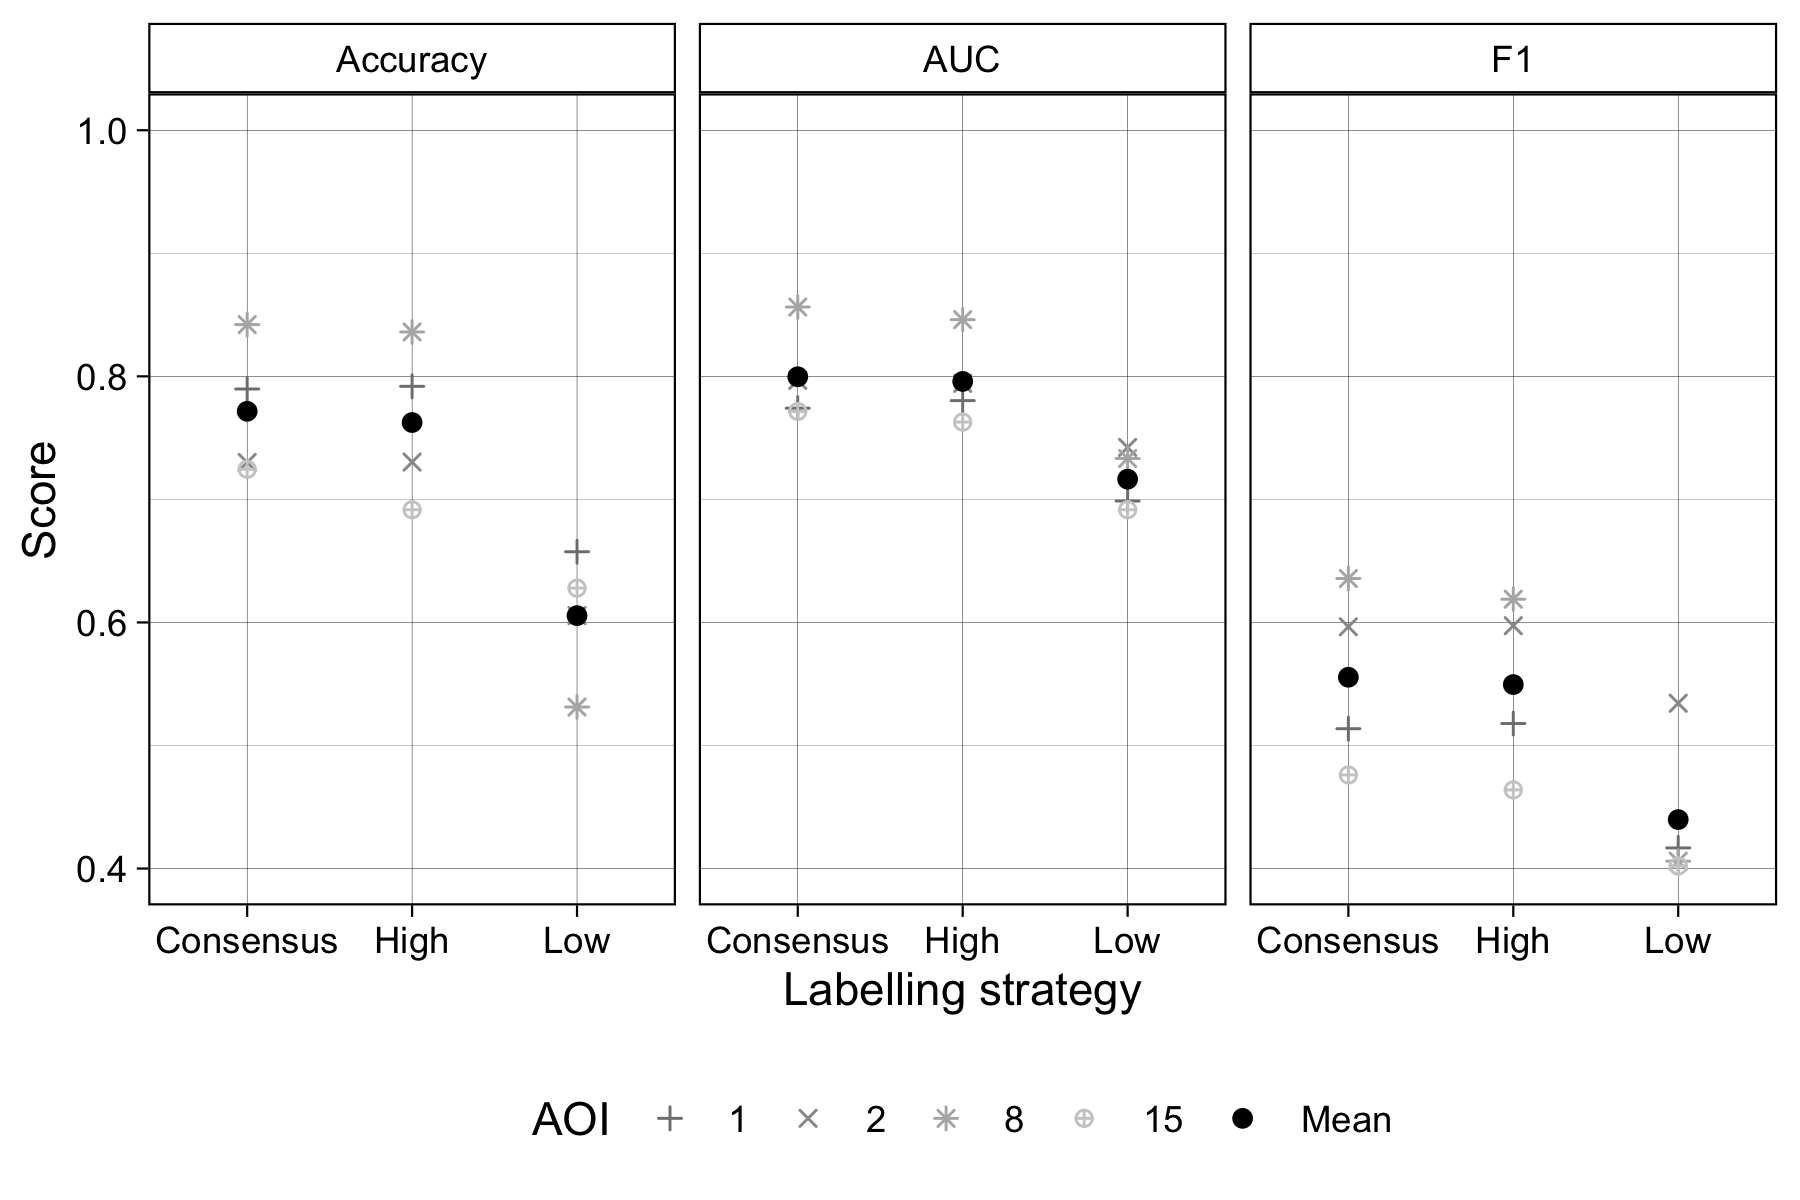
\includegraphics[width=0.9\linewidth]{figures/figure6} 

}

\caption{The distribution of croplands in Ghana. The main map shows the percentage of croplands in each 0.005 degree grid cell, derived from the predicted cropland probabilities. The insets  on the margins illustrate predicted probabilities (top map in each couplet) at original image resolution (0.000025 degrees) and segmented field boundaries overlaid on the dry season PlanetScope composite, for four separate tiles. Each tile's position is shown on the main map, and is color-coded to the boundary lines around its corresponding inset.}\label{fig:mainmap}
\end{figure}

Using the map reference sample and each map, we made two separate
estimates of the total cropland area in Ghana in 2018. The cropland
extent estimated from the field boundary map was 42,359 km\(^2\) (with a
margin of error of 4,395 km\(^2\)), or 17.1\% (15.4-18.9\%) of the
mapped area. The estimate from the per pixel map was 43,233 km\(^2\)
(margin of error = 4,904 km\(^2\)), or 17.6\% (15.6-19.6\%) of area.

The field boundary map provides additional information on how the
characteristics of croplands vary across Ghana, ranging from narrow,
strip-like fields in parts of AOI 15 (Figure \ref{fig:mainmap}'s lower
right inset) to more densely packed, less distinctly shaped fields in
AOI 5 (upper right inset in Figure \ref{fig:mainmap}). To explore how
field characteristics varied geographically, we mapped the average size
and total number of fields within each 0.05 degree tile grid (Figure
S15). These patterns generally correspond to those seen in the cropland
density map (Figure \ref{fig:mainmap}), with larger sizes and field
counts occurring where field densities are higher, although the biases
(relative to the validation labels) in both measures (Figures S13-14)
complicate interpretations of those variations. To minimize this
complication, we used the calculated biases to develop adjusted
estimates of field size and count (Table \ref{tab:sizentab}). These
adjusted estimates show that the typical field size in Ghana is 1.73 ha,
ranging from 0.96 in AOI 4 to 2.82 ha in AOI 4, with fields in the
forest zone AOIs (10, 11, 13, 14, 16) generally smaller than those in
the northern half of the country (Table \ref{tab:sizentab}). The
estimated total number of fields is 1,662,281, or 205 fields per tile
grid cells, varying from 108 fields/tile cell in AOI 4 to 399 in AOI 6.

\begin{table}[!h]

\caption{\label{tab:sizentab}The average size and total number of crop fields for each AOI and for Ghana overall. The original and bias-adjusted values for each measure are provided, as well as the total number of 0.05$^\circ$ degree tiles in each AOI.}
\centering
\begin{tabular}[t]{>{\raggedleft\arraybackslash}p{0.45in}>{\raggedleft\arraybackslash}p{0.45in}>{\raggedleft\arraybackslash}p{0.45in}>{\raggedleft\arraybackslash}p{0.85in}>{\raggedleft\arraybackslash}p{0.85in}>{\raggedleft\arraybackslash}p{0.85in}>{\raggedleft\arraybackslash}p{0.85in}>{\raggedleft\arraybackslash}p{0.85in}}
\toprule
AOI & N tiles & Size & Size (adj) & N & N / tile & N (adj) & N (adj) / tile\\
\midrule
1 & 777 & 3.71 & 1.26 & 97,822 & 126 & 127,580 & 164\\
2 & 597 & 7.66 & 1.96 & 87,666 & 147 & 120,651 & 202\\
3 & 501 & 8.24 & 2.18 & 108,819 & 217 & 104,422 & 208\\
4 & 465 & 2.44 & 2.82 & 26,276 & 57 & 50,163 & 108\\
5 & 400 & 4.24 & 2.09 & 43,290 & 108 & 53,756 & 134\\
\addlinespace
6 & 429 & 5.10 & 2.15 & 81,363 & 190 & 145,347 & 339\\
7 & 471 & 5.64 & 1.49 & 93,282 & 198 & 123,005 & 261\\
8 & 400 & 4.89 & 1.98 & 55,500 & 139 & 78,868 & 197\\
9 & 479 & 4.10 & 1.82 & 72,081 & 150 & 89,840 & 188\\
10 & 630 & 2.24 & 1.04 & 119,019 & 189 & 170,907 & 271\\
\addlinespace
11 & 400 & 3.65 & 1.52 & 52,510 & 131 & 94,709 & 237\\
12 & 471 & 3.44 & 1.77 & 44,667 & 95 & 52,947 & 112\\
13 & 627 & 0.84 & 0.96 & 67,996 & 108 & 125,368 & 200\\
14 & 400 & 1.09 & 2.72 & 56,006 & 140 & 101,767 & 254\\
15 & 548 & 4.95 & 1.54 & 75,752 & 138 & 105,681 & 193\\
\addlinespace
16 & 521 & 0.95 & 1.41 & 49,097 & 94 & 117,268 & 225\\
Ghana & 8,116 & 3.92 & 1.73 & 1,131,146 & 139 & 1,662,281 & 205\\
\bottomrule
\end{tabular}
\end{table}

\hypertarget{discussion}{%
\section{Discussion}\label{discussion}}

These results demonstrate a capability to map the characteristics of
smallholder-dominated cropping systems at high spatial resolution,
annual time steps, and national scales. The resulting maps provide an
updated and more granular view of the distribution and extent of
croplands in Ghana, complementing existing national to regional land
cover maps derived from moderate resolution imagery (Hackman et al.
2017, Xiong et al. 2017, ESA n.d.). Those prior studies estimated that
cropland covers 19.4 (Xiong et al. 2017) to 32\% (Hackman et al. 2017)
of Ghana in 2015. In contrast, our 2018 maps provide a raw estimate of
16.1-23.2\% cover (Table \ref{tab:mapaccuracy}), and our map reference
sample-based estimate was 17.1-17.6\%. Our results thus suggest that
Ghana's croplands are less extensive than those previous estimates.
However, this difference may arise from our use of a cropland definition
that excludes longer fallows and abandoned fields, which in some regions
may comprise over half of total cropland area (Tong et al. 2020).

In addition to this updated information on Ghana's cropland extent and
distribution, our results provide new insights into field size and
number at a national scale (Figures \ref{fig:mainmap}, S11-12). Previous
efforts to map smallholder field boundaries have either used \emph{in
situ} data collection (Carletto et al. 2013, 2015) or remote sensing
studies over relatively small (e.g. Forkuor et al. 2014, Persello et al.
2019) or discontiguous (Estes et al. 2016a) areas. The most extensive
studies to date enlisted crowdsourced volunteers to classify fields
visible within high resolution imagery sampled from virtual globes into
broad size categories (Fritz et al. 2015, Lesiv et al. 2019). Those
efforts included country-specific results for Ghana (n = 263), which
yield an average field size estimate of 5.33
ha\footnote{Obtained by calculating the weighted mean from the count of the five size classes and the mean of the hectare range provided for the four smallest size classes, and the lower bound of the size range provided for the largest size class. Data sourced from Table S3 in Lesiv et al. 2019.}.
This estimate exceeds our Ghana-wide average segment size (3.92 ha;
Table \ref{tab:sizentab}), but is closer to the mean (4.97 ha) within
AOIs 1-9, 12, and 15, which is where most of the crowdsourced sample
appears to have been collected. However, our bias-adjusted estimates of
1.73 (Ghana-wide) and 1.87 (AOIs 1-9, 12, and 15) ha were much smaller.

\hypertarget{map-accuracy-and-key-sources-of-error}{%
\subsection{Map accuracy and key sources of
error}\label{map-accuracy-and-key-sources-of-error}}

Although these maps provide valuable new information, they nevertheless
contain substantial errors. The overall accuracies (86.7-88\%, Table
\ref{tab:mapaccuracy}) are near the boundary of what might be considered
\emph{achievable} map accuracy (Elmes et al. 2020), given that we only
have \textasciitilde85\% confidence in our map reference sample, which
is our best estimate of the ``truth.'' However, accuracies for the
cropland class were much lower, falling between 62 (producer's) to 67
(user's) percent country-wide for the per-pixel map (Table
\ref{tab:mapaccuracy}), meaning the model produced substantial
commission and omission errors for this class. The segmented boundary
maps had fewer omission errors (producer's accuracy = 79\%), but higher
false positives (user's accuracy = 58.2\%). These accuracies are near
the middle to upper ranges of those reported for the cropland class in
other large-area mapping studies (Hackman et al. 2017, Xiong et al.
2017, Lesiv et al. 2017).

The patterns of accuracies within the cropland class varied by zone.
These zones largely align, albeit with some discrepancies, with the
country's agro-ecological zones (AEZs), thus the accuracy patterns may
be in part because some regions are simply more difficult to map.
Producer's accuracy for both maps was highest in the two northern zones
(1 and 2), which are primarily savannas (Figure S4), and lowest in zones
3 and 4, which are comprised of forest or coastal savannas. User's
accuracy followed a similar pattern, with the exception of Zone 3, which
had the highest user's accuracy, albeit from a very small sample.
Aligning the reference samples more precisely with agroecozone
boundaries (Figure S4B) provides further insight into error patterns
within the per-pixel map's cropland class (Table S4). Coastal savannas
in the southeast had the highest producer's and lowest user's accuracy,
perhaps because this region has high density cropland inter-mixed with
uncultivated areas that have low woody cover, which could help promote
commission error. Maps in the northern savannas had the best balance
between omission and commission error, and had the highest overall
user's accuracy. The transitional zone between forest and savanna had a
very low Producer's accuracy (21\%), which likely reflects the fact that
it was divided between several AOIs for mapping (Figure S4), and thus
was under-represented in the training samples, particularly in AOIs 10
and 11 (Figure S6B).

Beyond the errors linked to regional differences, several other
important factors contributed to map error. The first of these related
to the large mapping extent and image resolution. Given the goal of
developing a high resolution, country-scale map, the large data volume
constrained us to use a relatively small feature set and less than the
recommended tree number and depth (Maxwell et al. 2018) in our Random
Forests models, in order to limit computational costs. Previous work
found that Random Forests achieves much better performance on
small-scale croplands when trained on a much larger number of features
(Debats et al. 2016, Lebourgeois et al. 2017). However, applying such a
large feature set within the extent of our AOIs was not possible, as the
computing time and costs would have been several times
larger\footnote{Each active learning iteration ran for $\sim$4-8 hours on 800 CPUs, followed by a final $\sim$10-14 hours for prediction}.
This reduced the skill of the model, particularly when it came to
differentiating cropland from bare or sparsely vegetated patches, which
were common in many AOIs.

The inherent difficulty of the labelling task was another major limiting
factor. Our platform was designed to minimize label errors, but
determining croplands from non-croplands in these agricultural systems
can be difficult. Labellers had to evaluate multiple image sources and
to rely heavily on their judgment, which inevitably led to errors.
Interpretation was particularly hard where croplands and surrounding
landscapes had similar dry season reflectances, which was a particular
problem in the northernmost savannas. Smaller field sizes also
complicated labelling, as these become increasingly indistinct in the
\textasciitilde4 m PlanetScope composites. The difficulty of labelling
is reflected in the magnitude of the Bayesian Risk metrics (Figures
S10-11), and by the average assignment quality scores of each labeller
(71\%; Figure S9). Although prior work (Rodriguez-Galiano et al. 2012,
Mellor et al. 2015) found that Random Forests are robust to label error,
we found that it has substantial impact (Figure
\ref{fig:trainingimpact}), which suggests that improving label quality
is one of the most important factors in increasing model accuracy. Newer
models, such as convolutional neural networks, may be less sensitive to
label error, provided the error is random and the map reference samples
are of high quality (Burke et al. 2021). However, over many smallholder
systems training label errors will likely be biased in a particular
direction (e.g.~towards omission when fields are not easily
distinguished from the background), and our results show that reference
labels can have substantial uncertainty.

Image quality was another issue, although primarily in the forested
AOIs, where frequent cloud cover and the corresponding lower number of
available images resulted in lower quality composites (Figure
\ref{fig:imqual}), with more brightness artifacts and blur. This
impacted labellers' abilities to discern fields, and doubtless affected
model predictions. Little can be done to mitigate these errors, short of
confining imagery to the less cloudy dry season, which could reduce
model performance by removing the temporal contrast (Debats et al. 2016,
Defourny et al. 2019), or by adding radar data to the predictor set,
which would reduce map resolution. Composite quality could be improved
by using imagery from the same seasons over multiple years, but this
would undermine the goal of developing annual maps, while the dynamism
of the croplands would blur field boundaries within the imagery.

The final major source of error arose from the segmentation process. The
vectorized maps had high commission errors caused by uncertainties in
the Random Forests predictions. Model uncertainty meant that many pixels
in non-cropland areas had probabilities with values near 0.5. Segments
in these areas were retained if the average probability of intersected
pixels exceeded the 0.5 classification threshold. A more accurate
classifier would reduce such errors, as would a locally varying
classification threshold (e.g. Waldner and Diakogiannis 2020).
Over-merging was another source of error in the segmentation algorithm,
which led to overestimated field sizes and unrealistic shapes in some
areas, particularly in high density croplands (e.g.~in AOIs 2 and 8;
Figure \ref{fig:mainmap}) where boundaries between adjacent fields were
indistinct in the imagery. Preventing merging could help in such cases,
but potentially lead to over-segmentation, thereby underestimating field
sizes.

\hypertarget{error-mitigation-features}{%
\subsection{Error mitigation features}\label{error-mitigation-features}}

Despite these numerous source of errors, our approach was effective in
mitigating several of these error sources. Label quality assessment and
consensus labelling were the most effective error mitigation tools.
Label quality scores allowed us to quantify the impact of label error on
model performance (Figure \ref{fig:trainingimpact}), while consensus
labels produced maps that were more accurate than they would have been
if we had relied on individually generated labels. The quality scores
also helped to improve the overall accuracy of consensus labels, by
placing higher weight on the work of more accurate labellers. In
addition to these benefits, label quality scores (Figure S9) also
allowed us to select the labels most likely to accurately capture field
sizes and numbers, which we used to estimated and correct the biases in
these two measures derived from the segmented field boundaries.

Active learning improved overall model performance relative to
randomized training site selection, in line with findings from two
recent efforts (Debats et al. 2017, Hamrouni et al. 2021). Although the
relative performance gains that we observed were smaller (e.g. Debats et
al. (2017) 29\% higher model performance after one iteration, and 8\%
higher on the final iterations), those comparisons were made by starting
with a training sample that was \textless1/10 the size of ours. Our
large starter sample meant that the models were substantially trained
before they were exposed to actively selected labels, thereby diluting
their impact on performance. Nevertheless, we found higher performance
from active learning, most notably in the F1 score (Figure S8), a
balanced performance metric, which further demonstrates its
effectiveness.

The detail, temporal precision, and large extent of our maps was enabled
by the ability to process PlanetScope data, which is currently the only
source of sub-5 meter imagery with daily coverage (McCabe et al. 2017).
Daily revisits are important for creating seasonal composites within a
single year over cloudy areas. The compositing technique we developed
allowed us to develop a complete image catalog for the country
representing the two seasons for 2018 agricultural year. Although
Sentinel-2 is free, has better radiometric quality, and has sufficient
spatial resolution (10 m) to accurately classify small-scale
agricultural systems (e.g. Defourny et al. 2019, Kerner et al. 2020),
its 5-day interval may be too infrequent to generate cloud-free
composites during the growing season over southern Ghana. Sentinel-1 is
not affected by the same problem, but labeling fields in radar images is
more challenging.

\hypertarget{lingering-questions}{%
\subsection{Lingering questions}\label{lingering-questions}}

Several potential issues not addressed in our assessment merit further
exploration. One of these was the degree of correspondence between
image- and ground-collected labels. However, such comparisons may reveal
unresolvable discrepancies between the two perspectives. The highly
dynamic nature of these agricultural systems means that relatively
narrow differences between the dates of ground- and image-based label
collection can lead to substantial disagreement, simply because the
fields themselves may have shifted during the interval (Elmes et al.
2020). These discrepancies can be exacerbated by the definition used to
determine what constitutes a field, which might vary on the ground
depending on who is being asked, or who is doing the collecting. These
factors suggest that difference between ground- and image-collected
labels would not necessarily indicate how far image labellers were from
the ``truth.'' Nevertheless, a comparison against ground data would help
to assess how accurately image-collected labels capture the typical size
of fields, and thus merits further investigation.

The temporal discrepancies mentioned above (and discussed in Elmes et
al. 2020) are another reason why we chose not to label on basemap
imagery (in addition to restrictive usage terms), which is typically
several years old (Lesiv et al. 2018). However, we did not assess
whether the higher label accuracy one might achieve by digitizing on a
\textless1-2 m resolution basemap would offset model errors caused by
temporal mismatches.

Another potential issue is the degree to which our assessment of label
error on model performance (Figure \ref{fig:trainingimpact}) was
influenced by the validation dataset we used, which was based on
consensus labels. This could have confounded the analysis, particularly
when comparing the consensus label-trained models with those trained
with the most accurate individual labels. However, a visual assessment
of the resulting probability maps confirms that models trained with the
consensus and most accurate individual labels were more precise than the
model trained with lower quality labels (Figure S12).

\hypertarget{broader-applications}{%
\subsection{Broader applications}\label{broader-applications}}

This work demonstrates a proof of concept for developing high
resolution, annual maps of smallholder-dominated croplands at national
to regional scales, using an approach that follows recommended best
practices for training and assessing machine learning models (Elmes et
al. 2020). This approach can be readily updated to integrate
improvements, such as newer machine learning models. Beyond providing
valuable insights into field characteristics, field boundary maps can
help improve remote estimation of crop areas and yield (e.g. Estes et
al. 2013), and provide deeper insights into important socioeconomic
aspects of agricultural systems, such as the relationships between
agricultural productivity and farm size (Feder 1985, Carletto et al.
2013, Desiere and Jolliffe 2018). Such maps will be important for
understanding the rapid agricultural change that is currently occurring
in Africa.

\hypertarget{data-availability-and-usage}{%
\subsection{Data availability and
usage}\label{data-availability-and-usage}}

The maps presented here are a version 1 product that is freely available
to use, along with its underlying code (see SI). In their current form,
they may be useful for a variety of research applications. For example,
analyzing the distributions of values in the probability maps may
provide additional insight into the relative extents of active versus
fallow croplands (Tong et al. 2020). However, use of these data,
particularly for decision-making processes (e.g.~cropped area
estimates), should be careful to account for the reported errors
(Olofsson et al. 2014, Stehman and Foody 2019).

\hypertarget{acknowledgements}{%
\section{Acknowledgements}\label{acknowledgements}}

The primary support for this work was provided by Omidyar Network's
Property Rights Initiative, now PLACE. Additional support was provided
by NASA (80NSSC18K0158), the National Science Foundation (SES-1801251;
SES-1832393), and Princeton University. Computing support was provided
by the AWS Cloud Credits for Research program and the Amazon
Sustainability Data Initiative. Azavea provided significant
contributions in engineering the machine learning pipeline. We thank
Meridia for providing information about local cropping systems and the
characteristics of fields, and Radiant Earth Foundation for advice and
guidance regarding machine learning best practices. We thank Manushi
Trivedi, Sitian Xiong, and Tammy Woodard for their contributions to the
underlying datasets and methods, and Michelle Gathigi, Omar Shehe, and
Primoz Kovacic for support and management of the labelling efforts.

\hypertarget{references}{%
\section{References}\label{references}}

\singlespace

\hypertarget{refs}{}
\begin{CSLReferences}{1}{0}
\leavevmode\hypertarget{ref-azaveaRasterFoundry2020}{}%
Azavea. 2020. Raster {Foundry}.
https://github.com/raster-foundry/raster-foundry.

\leavevmode\hypertarget{ref-BeyCollectEarthLand2016}{}%
Bey, A., A. Sánchez-Paus Díaz, D. Maniatis, G. Marchi, D. Mollicone, S.
Ricci, J.-F. Bastin, R. Moore, S. Federici, M. Rezende, C. Patriarca, R.
Turia, G. Gamoga, H. Abe, E. Kaidong, and G. Miceli. 2016. Collect
{Earth}: {Land Use} and {Land Cover Assessment} through {Augmented
Visual Interpretation}. Remote Sensing 8:807.

\leavevmode\hypertarget{ref-boschettiAnalysisConflictOmission2004}{}%
Boschetti, L., S. P. Flasse, and P. A. Brivio. 2004. Analysis of the
conflict between omission and commission in low spatial resolution
dichotomic thematic products: {The Pareto Boundary}. Remote Sensing of
Environment 91:280--292.

\leavevmode\hypertarget{ref-BreimanRandomForests2001}{}%
Breiman, L. 2001. Random {Forests}. Machine Learning 45:5--32.

\leavevmode\hypertarget{ref-bullockThreeDecadesLand2021}{}%
Bullock, E. L., S. P. Healey, Z. Yang, P. Oduor, N. Gorelick, S. Omondi,
E. Ouko, and W. B. Cohen. 2021. Three {Decades} of {Land Cover Change}
in {East Africa}. Land 10:150.

\leavevmode\hypertarget{ref-burkeUsingSatelliteImagery2021}{}%
Burke, M., A. Driscoll, D. B. Lobell, and S. Ermon. 2021. Using
satellite imagery to understand and promote sustainable development.
Science 371.

\leavevmode\hypertarget{ref-CarlettoGuesstimatesGPStimatesLand2015}{}%
Carletto, C., S. Gourlay, and P. Winters. 2015. From {Guesstimates} to
{GPStimates}: {Land Area Measurement} and {Implications} for
{Agricultural Analysis}. Journal of African Economies 24:593--628.

\leavevmode\hypertarget{ref-CarlettoFactartifactimpact2013}{}%
Carletto, C., S. Savastano, and A. Zezza. 2013. Fact or artifact: {The}
impact of measurement errors on the farm size{}productivity
relationship. Journal of Development Economics 103:254--261.

\leavevmode\hypertarget{ref-ChenGloballandcover2015}{}%
Chen, J., J. Chen, A. Liao, X. Cao, L. Chen, X. Chen, C. He, G. Han, S.
Peng, M. Lu, W. Zhang, X. Tong, and J. Mills. 2015. Global land cover
mapping at 30 m resolution: {A POK}-based operational approach. ISPRS
Journal of Photogrammetry and Remote Sensing 103:7--27.

\leavevmode\hypertarget{ref-cohnImprovingGeneralizationActive1994}{}%
Cohn, D., L. Atlas, and R. Ladner. 1994. Improving generalization with
active learning. Machine Learning 15:201--221.

\leavevmode\hypertarget{ref-Darkmodifiablearealunit2007}{}%
Dark, S. J., and D. Bram. 2007. The modifiable areal unit problem
({MAUP}) in physical geography. Progress in Physical Geography
31:471--479.

\leavevmode\hypertarget{ref-davisTropicalForestLoss2020}{}%
Davis, K. F., H. I. Koo, J. Dell'Angelo, P. D'Odorico, L. Estes, L. J.
Kehoe, M. Kharratzadeh, T. Kuemmerle, D. Machava, A. de J. R. Pais, N.
Ribeiro, M. C. Rulli, and M. Tatlhego. 2020. Tropical forest loss
enhanced by large-scale land acquisitions. Nature Geoscience:1--7.

\leavevmode\hypertarget{ref-DebatsIntegratingactivelearning2017}{}%
Debats, S. R., L. D. Estes, D. R. Thompson, and K. K. Caylor. 2017.
Integrating active learning and crowdsourcing into large-scale
supervised landcover mapping algorithms. {PeerJ Preprints}.

\leavevmode\hypertarget{ref-Debatsgeneralizedcomputervision2016}{}%
Debats, S. R., D. Luo, L. D. Estes, T. J. Fuchs, and K. K. Caylor. 2016.
A generalized computer vision approach to mapping crop fields in
heterogeneous agricultural landscapes. Remote Sensing of Environment
179:210--221.

\leavevmode\hypertarget{ref-Defournyrealtimeagriculturemonitoring2019}{}%
Defourny, P., S. Bontemps, N. Bellemans, C. Cara, G. Dedieu, E.
Guzzonato, O. Hagolle, J. Inglada, L. Nicola, T. Rabaute, M. Savinaud,
C. Udroiu, S. Valero, A. Bégué, J.-F. Dejoux, A. El Harti, J. Ezzahar,
N. Kussul, K. Labbassi, V. Lebourgeois, Z. Miao, T. Newby, A. Nyamugama,
N. Salh, A. Shelestov, V. Simonneaux, P. S. Traore, S. S. Traore, and B.
Koetz. 2019. Near real-time agriculture monitoring at national scale at
parcel resolution: {Performance} assessment of the {Sen2}-{Agri}
automated system in various cropping systems around the world. Remote
Sensing of Environment 221:551--568.

\leavevmode\hypertarget{ref-desiereLandProductivityPlot2018}{}%
Desiere, S., and D. Jolliffe. 2018. Land productivity and plot size:
{Is} measurement error driving the inverse relationship? Journal of
Development Economics 130:84--98.

\leavevmode\hypertarget{ref-DruschSentinel2ESAOptical2012}{}%
Drusch, M., U. Del Bello, S. Carlier, O. Colin, V. Fernandez, F. Gascon,
B. Hoersch, C. Isola, P. Laberinti, P. Martimort, A. Meygret, F. Spoto,
O. Sy, F. Marchese, and P. Bargellini. 2012. Sentinel-2: {ESA}'s
{Optical High}-{Resolution Mission} for {GMES Operational Services}.
Remote Sensing of Environment 120:25--36.

\leavevmode\hypertarget{ref-DwyerAnalysisReadyData2018}{}%
Dwyer, J. L., D. P. Roy, B. Sauer, C. B. Jenkerson, H. K. Zhang, and L.
Lymburner. 2018. Analysis {Ready Data}: {Enabling Analysis} of the
{Landsat Archive}. Remote Sensing 10:1363.

\leavevmode\hypertarget{ref-ElmesAccountingtrainingdata2020}{}%
Elmes, A., H. Alemohammad, R. Avery, K. Caylor, J. R. Eastman, L.
Fishgold, M. A. Friedl, M. Jain, D. Kohli, J. C. Laso Bayas, D. Lunga,
J. L. McCarty, R. G. Pontius, A. B. Reinmann, J. Rogan, L. Song, H.
Stoynova, S. Ye, Z.-F. Yi, and L. Estes. 2020. Accounting for training
data error in machine learning applied to {Earth Observations}. Remote
Sensing 12:1034.

\leavevmode\hypertarget{ref-ESAESACCILAND}{}%
ESA. (n.d.). {ESA CCI LAND COVER} {} {S2} prototype {Land Cover} 20m map
of {Africa} 2016. http://2016africalandcover20m.esrin.esa.int/.

\leavevmode\hypertarget{ref-Esteslargeareaspatiallycontinuous2018}{}%
Estes, L., P. Chen, S. Debats, T. Evans, S. Ferreira, T. Kuemmerle, G.
Ragazzo, J. Sheffield, A. Wolf, E. Wood, and K. Caylor. 2018. A
large-area, spatially continuous assessment of land cover map error and
its impact on downstream analyses. Global Change Biology 24:322--337.

\leavevmode\hypertarget{ref-EstesProjectedclimateimpacts2013}{}%
Estes, L. D., H. Beukes, B. A. Bradley, S. R. Debats, M. Oppenheimer, A.
C. Ruane, R. Schulze, and M. Tadross. 2013. Projected climate impacts to
{South African} maize and wheat production in 2055: A comparison of
empirical and mechanistic modeling approaches. Global Change Biology
19:3762--3774.

\leavevmode\hypertarget{ref-Estesplatformcrowdsourcingcreation2016}{}%
Estes, L. D., D. McRitchie, J. Choi, S. Debats, T. Evans, W. Guthe, D.
Luo, G. Ragazzo, R. Zempleni, and K. K. Caylor. 2016a. A platform for
crowdsourcing the creation of representative, accurate landcover maps.
Environmental Modelling \& Software 80:41--53.

\leavevmode\hypertarget{ref-EstesReconcilingagriculturecarbon2016}{}%
Estes, L. D., T. Searchinger, M. Spiegel, D. Tian, S. Sichinga, M.
Mwale, L. Kehoe, T. Kuemmerle, A. Berven, N. Chaney, J. Sheffield, E. F.
Wood, and K. K. Caylor. 2016b. Reconciling agriculture, carbon and
biodiversity in a savannah transformation frontier. Phil. Trans. R. Soc.
B 371:20150316.

\leavevmode\hypertarget{ref-federRelationFarmSize1985}{}%
Feder, G. 1985. The relation between farm size and farm productivity:
{The} role of family labor, supervision and credit constraints. Journal
of Development Economics 18:297--313.

\leavevmode\hypertarget{ref-forkuorIntegrationOpticalSynthetic2014}{}%
Forkuor, G., C. Conrad, M. Thiel, T. Ullmann, and E. Zoungrana. 2014.
Integration of {Optical} and {Synthetic Aperture Radar Imagery} for
{Improving Crop Mapping} in {Northwestern Benin}, {West Africa}. Remote
Sensing 6:6472--6499.

\leavevmode\hypertarget{ref-FourieBetterCropEstimates2009}{}%
Fourie, A. 2009. Better {Crop Estimates} in {South Africa}. ArcUser
Online.

\leavevmode\hypertarget{ref-FritzGeoWikionlineplatform2012}{}%
Fritz, S., I. McCallum, C. Schill, C. Perger, L. See, D. Schepaschenko,
M. van der Velde, F. Kraxner, and M. Obersteiner. 2012. Geo-{Wiki}: {An}
online platform for improving global land cover. Environmental Modelling
\& Software 31:110--123.

\leavevmode\hypertarget{ref-FritzHighlightingcontinueduncertainty2011}{}%
Fritz, S., L. See, I. McCallum, C. Schill, M. Obersteiner, M. van der
Velde, H. Boettcher, P. Havlík, and F. Achard. 2011. Highlighting
continued uncertainty in global land cover maps for the user community.
Environmental Research Letters 6:044005.

\leavevmode\hypertarget{ref-FritzMappingglobalcropland2015}{}%
Fritz, S., L. See, I. McCallum, L. You, A. Bun, E. Moltchanova, M.
Duerauer, F. Albrecht, C. Schill, C. Perger, P. Havlik, A. Mosnier, P.
Thornton, U. Wood-Sichra, M. Herrero, I. Becker-Reshef, C. Justice, M.
Hansen, P. Gong, S. Abdel Aziz, A. Cipriani, R. Cumani, G. Cecchi, G.
Conchedda, S. Ferreira, A. Gomez, M. Haffani, F. Kayitakire, J.
Malanding, R. Mueller, T. Newby, A. Nonguierma, A. Olusegun, S. Ortner,
D. R. Rajak, J. Rocha, D. Schepaschenko, M. Schepaschenko, A. Terekhov,
A. Tiangwa, C. Vancutsem, E. Vintrou, W. Wenbin, M. van der Velde, A.
Dunwoody, F. Kraxner, and M. Obersteiner. 2015. Mapping global cropland
and field size. Global Change Biology 21:1980--1992.

\leavevmode\hypertarget{ref-FritzComparisonglobalregional2010}{}%
Fritz, S., L. See, and F. Rembold. 2010. Comparison of global and
regional land cover maps with statistical information for the
agricultural domain in {Africa}. International Journal of Remote Sensing
31:2237--2256.

\leavevmode\hypertarget{ref-Fritzneedimprovedmaps2013}{}%
Fritz, S., L. See, L. You, C. Justice, I. Becker-Reshef, L. Bydekerke,
R. Cumani, P. Defourny, K. Erb, J. Foley, S. Gilliams, P. Gong, M.
Hansen, T. Hertel, M. Herold, M. Herrero, F. Kayitakire, J. Latham, O.
Leo, I. McCallum, M. Obersteiner, N. Ramankutty, J. Rocha, H. Tang, P.
Thornton, C. Vancutsem, M. van der Velde, S. Wood, and C. Woodcock.
2013. The need for improved maps of global cropland. Eos, Transactions
American Geophysical Union 94:31--32.

\leavevmode\hypertarget{ref-GibbsTropicalforestswere2010}{}%
Gibbs, H. K., A. S. Ruesch, F. Achard, M. K. Clayton, P. Holmgren, N.
Ramankutty, and J. A. Foley. 2010. Tropical forests were the primary
sources of new agricultural land in the 1980s and 1990s. Proceedings of
the National Academy of Sciences 107:16732--16737.

\leavevmode\hypertarget{ref-GorelickGoogleEarthEngine2017}{}%
Gorelick, N., M. Hancher, M. Dixon, S. Ilyushchenko, D. Thau, and R.
Moore. 2017. Google {Earth Engine}: {Planetary}-scale geospatial
analysis for everyone. Remote Sensing of Environment 202:18--27.

\leavevmode\hypertarget{ref-hackmanNewLandcoverMaps2017}{}%
Hackman, K. O., P. Gong, and J. Wang. 2017. New land-cover maps of
{Ghana} for 2015 using {Landsat} 8 and three popular classifiers for
biodiversity assessment. International Journal of Remote Sensing
38:4008--4021.

\leavevmode\hypertarget{ref-hamrouniLocalGlobalTransfer2021}{}%
Hamrouni, Y., E. Paillassa, V. Chéret, C. Monteil, and D. Sheeren. 2021.
From local to global: {A} transfer learning-based approach for mapping
poplar plantations at national scale using {Sentinel}-2. ISPRS Journal
of Photogrammetry and Remote Sensing 171:76--100.

\leavevmode\hypertarget{ref-HouborgDailyRetrievalNDVI2018}{}%
Houborg, R., and M. McCabe. 2018. Daily {Retrieval} of {NDVI} and {LAI}
at 3 m {Resolution} via the {Fusion} of {CubeSat}, {Landsat}, and {MODIS
Data}. Remote Sensing 10:890.

\leavevmode\hypertarget{ref-KansangaTraditionalagriculturetransition2019}{}%
Kansanga, M., P. Andersen, D. Kpienbaareh, S. Mason-Renton, K. Atuoye,
Y. Sano, R. Antabe, and I. Luginaah. 2019. Traditional agriculture in
transition: Examining the impacts of agricultural modernization on
smallholder farming in {Ghana} under the new {Green Revolution}.
International Journal of Sustainable Development \& World Ecology
26:11--24.

\leavevmode\hypertarget{ref-kehoeNatureRiskFuture2017}{}%
Kehoe, L., A. Romero-Muñoz, L. Estes, H. Kreft, E. Polaina, and T.
Kuemmerle. 2017. Nature at risk under future agricultural expansion and
intensification. Nature Ecology and Evolution 1:1129--1135.

\leavevmode\hypertarget{ref-kernerRapidResponseCrop2020}{}%
Kerner, H., G. Tseng, I. Becker-Reshef, C. Nakalembe, B. Barker, B.
Munshell, M. Paliyam, and M. Hosseini. 2020. Rapid {Response Crop Maps}
in {Data Sparse Regions}. arXiv:2006.16866 {[}cs, eess{]}.

\leavevmode\hypertarget{ref-lebourgeoisCombinedRandomForest2017}{}%
Lebourgeois, V., S. Dupuy, É. Vintrou, M. Ameline, S. Butler, and A.
Bégué. 2017. A {Combined Random Forest} and {OBIA Classification Scheme}
for {Mapping Smallholder Agriculture} at {Different Nomenclature Levels
Using Multisource Data} ({Simulated Sentinel}-2 {Time Series}, {VHRS}
and {DEM}). Remote Sensing 9:259.

\leavevmode\hypertarget{ref-LesivEvaluationESACCI2017}{}%
Lesiv, M., S. Fritz, I. McCallum, N. Tsendbazar, M. Herold, J.-F. Pekel,
M. Buchhorn, B. Smets, and R. Van De Kerchove. 2017, November.
Evaluation of {ESA CCI} prototype land cover map at 20m. Monograph,
http://pure.iiasa.ac.at/id/eprint/14979/.

\leavevmode\hypertarget{ref-lesivEstimatingGlobalDistribution2019}{}%
Lesiv, M., J. C. Laso Bayas, L. See, M. Duerauer, D. Dahlia, N. Durando,
R. Hazarika, P. Kumar Sahariah, M. Vakolyuk, V. Blyshchyk, A. Bilous, A.
Perez-Hoyos, S. Gengler, R. Prestele, S. Bilous, I. ul H. Akhtar, K.
Singha, S. B. Choudhury, T. Chetri, Ž. Malek, K. Bungnamei, A. Saikia,
D. Sahariah, W. Narzary, O. Danylo, T. Sturn, M. Karner, I. McCallum, D.
Schepaschenko, E. Moltchanova, D. Fraisl, I. Moorthy, and S. Fritz.
2019. Estimating the global distribution of field size using
crowdsourcing. Global Change Biology 25:174--186.

\leavevmode\hypertarget{ref-LesivCharacterizingspatialtemporal2018}{}%
Lesiv, M., L. See, J. Laso Bayas, T. Sturn, D. Schepaschenko, M. Karner,
I. Moorthy, I. McCallum, and S. Fritz. 2018. Characterizing the spatial
and temporal availability of very high resolution satellite imagery in
{Google Earth} and {Microsoft Bing} maps as a source of reference data.
Land 7:118.

\leavevmode\hypertarget{ref-levinFarmSizeLandscape2006}{}%
Levin, G. 2006. Farm size and landscape composition in relation to
landscape changes in {Denmark}. Geografisk Tidsskrift-Danish Journal of
Geography 106:45--59.

\leavevmode\hypertarget{ref-LickerMindgaphow2010}{}%
Licker, R., M. Johnston, J. A. Foley, C. Barford, C. J. Kucharik, C.
Monfreda, and N. Ramankutty. 2010. Mind the gap: How do climate and
agricultural management explain the {`yield gap'} of croplands around
the world? Global Ecology and Biogeography 19:769--782.

\leavevmode\hypertarget{ref-lobellCropYieldGaps2009}{}%
Lobell, D. B., K. G. Cassman, and C. B. Field. 2009. Crop {Yield Gaps}:
{Their Importance}, {Magnitudes}, and {Causes}. Annual Review of
Environment and Resources 34:179--204.

\leavevmode\hypertarget{ref-maDeepLearningRemote2019}{}%
Ma, L., Y. Liu, X. Zhang, Y. Ye, G. Yin, and B. A. Johnson. 2019. Deep
learning in remote sensing applications: {A} meta-analysis and review.
ISPRS Journal of Photogrammetry and Remote Sensing 152:166--177.

\leavevmode\hypertarget{ref-MaxwellImplementationmachinelearningclassification2018}{}%
Maxwell, A. E., T. A. Warner, and F. Fang. 2018. Implementation of
machine-learning classification in remote sensing: An applied review.
International Journal of Remote Sensing 39:2784--2817.

\leavevmode\hypertarget{ref-McCabefutureEarthobservation2017}{}%
McCabe, M. F., M. Rodell, D. E. Alsdorf, D. G. Miralles, R. Uijlenhoet,
W. Wagner, A. Lucieer, R. Houborg, N. E. C. Verhoest, T. E. Franz, J.
Shi, H. Gao, and E. F. Wood. 2017. The future of {Earth} observation in
hydrology. Hydrology and Earth System Sciences 21:3879--3914.

\leavevmode\hypertarget{ref-mellorExploringIssuesTraining2015}{}%
Mellor, A., S. Boukir, A. Haywood, and S. Jones. 2015. Exploring issues
of training data imbalance and mislabelling on random forest performance
for large area land cover classification using the ensemble margin.
ISPRS Journal of Photogrammetry and Remote Sensing 105:155--168.

\leavevmode\hypertarget{ref-morrisAwakeningAfricaSleeping2009}{}%
Morris, M., and D. Byerlee. 2009. Awakening {Africa}'s {Sleeping Giant}.
{World Bank and FAO}, {Washington, DC}.

\leavevmode\hypertarget{ref-muellerClosingYieldGaps2012}{}%
Mueller, N. D., J. S. Gerber, M. Johnston, D. K. Ray, N. Ramankutty, and
J. A. Foley. 2012. Closing yield gaps through nutrient and water
management. Nature 490:254--257.

\leavevmode\hypertarget{ref-neubertCompactWatershedPreemptive2014}{}%
Neubert, P., and P. Protzel. 2014. Compact {Watershed} and {Preemptive
SLIC}: {On Improving Trade}-offs of {Superpixel Segmentation
Algorithms}. Pages 996--1001 2014 22nd {International Conference} on
{Pattern Recognition}. {IEEE}, {Stockholm, Sweden}.

\leavevmode\hypertarget{ref-OlofssonGoodpracticesestimating2014}{}%
Olofsson, P., G. M. Foody, M. Herold, S. V. Stehman, C. E. Woodcock, and
M. A. Wulder. 2014. Good practices for estimating area and assessing
accuracy of land change. Remote Sensing of Environment 148:42--57.

\leavevmode\hypertarget{ref-OlofssonMakingbetteruse2013}{}%
Olofsson, P., G. M. Foody, S. V. Stehman, and C. E. Woodcock. 2013.
Making better use of accuracy data in land change studies: {Estimating}
accuracy and area and quantifying uncertainty using stratified
estimation. Remote Sensing of Environment 129:122--131.

\leavevmode\hypertarget{ref-Openshawmillioncorrelationcoefficients1979}{}%
Openshaw, S., and P. J. Taylor. 1979. A million or so correlation
coefficients: Three experiments on the modifiable areal unit problem.
Statistical applications in the spatial sciences 21:127--144.

\leavevmode\hypertarget{ref-perselloDelineationAgriculturalFields2019}{}%
Persello, C., V. A. Tolpekin, J. R. Bergado, and R. A. de By. 2019.
Delineation of agricultural fields in smallholder farms from satellite
images using fully convolutional networks and combinatorial grouping.
Remote Sensing of Environment 231:111253.

\leavevmode\hypertarget{ref-planetteamPlanetApplicationProgram2018}{}%
PlanetTeam. 2018. Planet application program interface: In space for
life on {Earth}. {https://api.planet.com}, {San Francisco, CA}.

\leavevmode\hypertarget{ref-Pontiustotaloperatingcharacteristic2014}{}%
Pontius, R. G., and K. Si. 2014. The total operating characteristic to
measure diagnostic ability for multiple thresholds. International
Journal of Geographical Information Science 28:570--583.

\leavevmode\hypertarget{ref-qiuCirrusCloudsThat2020}{}%
Qiu, S., Z. Zhu, and C. E. Woodcock. 2020. Cirrus clouds that adversely
affect {Landsat} 8 images: {What} are they and how to detect them?
Remote Sensing of Environment 246:111884.

\leavevmode\hypertarget{ref-rodriguez-galianoAssessmentEffectivenessRandom2012}{}%
Rodriguez-Galiano, V. F., B. Ghimire, J. Rogan, M. Chica-Olmo, and J. P.
Rigol-Sanchez. 2012. An assessment of the effectiveness of a random
forest classifier for land-cover classification. ISPRS Journal of
Photogrammetry and Remote Sensing 67:93--104.

\leavevmode\hypertarget{ref-royGlobalAnalysisTemporal2021}{}%
Roy, D. P., H. Huang, R. Houborg, and V. S. Martins. 2021. A global
analysis of the temporal availability of {PlanetScope} high spatial
resolution multi-spectral imagery. Remote Sensing of Environment
264:112586.

\leavevmode\hypertarget{ref-RulliFoodappropriationlarge2014}{}%
Rulli, M. C., and P. D'Odorico. 2014. Food appropriation through large
scale land acquisitions. Environmental Research Letters 9:064030.

\leavevmode\hypertarget{ref-SambergSubnationaldistributionaverage2016}{}%
Samberg, L. H., J. S. Gerber, N. Ramankutty, M. Herrero, and P. C. West.
2016. Subnational distribution of average farm size and smallholder
contributions to global food production. Environmental Research Letters
11:124010.

\leavevmode\hypertarget{ref-SearchingerHighcarbonbiodiversity2015}{}%
Searchinger, T. D., L. Estes, P. K. Thornton, T. Beringer, A.
Notenbaert, D. Rubenstein, R. Heimlich, R. Licker, and M. Herrero. 2015.
High carbon and biodiversity costs from converting {Africa}'s wet
savannahs to cropland. Nature Climate Change 5:481--486.

\leavevmode\hypertarget{ref-searchingerCreatingSustainableFood2019}{}%
Searchinger, T., R. Waite, C. Hanson, J. Ranganathan, P. Dumas, E.
Matthews, and C. Klirs. 2019. Creating a sustainable food future: {A}
menu of solutions to feed nearly 10 billion people by 2050. {Final}
report. {WRI}.

\leavevmode\hypertarget{ref-StehmanKeyissuesrigorous2019}{}%
Stehman, S. V., and G. M. Foody. 2019. Key issues in rigorous accuracy
assessment of land cover products. Remote Sensing of Environment
231:111199.

\leavevmode\hypertarget{ref-sulla-menasheHierarchicalMappingAnnual2019}{}%
Sulla-Menashe, D., J. M. Gray, S. P. Abercrombie, and M. A. Friedl.
2019. Hierarchical mapping of annual global land cover 2001 to present:
{The MODIS Collection} 6 {Land Cover} product. Remote Sensing of
Environment 222:183--194.

\leavevmode\hypertarget{ref-Tongforgottenlanduse2020}{}%
Tong, X., M. Brandt, P. Hiernaux, S. Herrmann, L. V. Rasmussen, K.
Rasmussen, F. Tian, T. Tagesson, W. Zhang, and R. Fensholt. 2020. The
forgotten land use class: {Mapping} of fallow fields across the {Sahel}
using {Sentinel}-2. Remote Sensing of Environment 239:111598.

\leavevmode\hypertarget{ref-tuiaSurveyActiveLearning2011}{}%
Tuia, D., M. Volpi, L. Copa, M. Kanevski, and J. Munoz-Mari. 2011. A
{Survey} of {Active Learning Algorithms} for {Supervised Remote Sensing
Image Classification}. IEEE Journal of Selected Topics in Signal
Processing 5:606--617.

\leavevmode\hypertarget{ref-vanvlietThereContinuingRationale2013}{}%
Van Vliet, N., O. Mertz, T. Birch-Thomsen, and B. Schmook. 2013. Is
{There} a {Continuing Rationale} for {Swidden Cultivation} in the 21st
{Century}? Human Ecology 41:1--5.

\leavevmode\hypertarget{ref-visvalingamLineGeneralisationRepeated1993}{}%
Visvalingam, M., and J. D. Whyatt. 1993. Line generalisation by repeated
elimination of points. The Cartographic Journal 30:46--51.

\leavevmode\hypertarget{ref-waldnerDeepLearningEdge2020}{}%
Waldner, F., and F. I. Diakogiannis. 2020. Deep learning on edge:
{Extracting} field boundaries from satellite images with a convolutional
neural network. Remote Sensing of Environment 245:111741.

\leavevmode\hypertarget{ref-WaldnerConflationexpertcrowd2019}{}%
Waldner, F., A. Schucknecht, M. Lesiv, J. Gallego, L. See, A.
Pérez-Hoyos, R. d'Andrimont, T. de Maet, J. C. L. Bayas, S. Fritz, O.
Leo, H. Kerdiles, M. Díez, K. Van Tricht, S. Gilliams, A. Shelestov, M.
Lavreniuk, M. Simões, R. Ferraz, B. Bellón, A. Bégué, G. Hazeu, V.
Stonacek, J. Kolomaznik, J. Misurec, S. R. Verón, D. de Abelleyra, D.
Plotnikov, L. Mingyong, M. Singha, P. Patil, M. Zhang, and P. Defourny.
2019. Conflation of expert and crowd reference data to validate global
binary thematic maps. Remote Sensing of Environment 221:235--246.

\leavevmode\hypertarget{ref-WilsonRemotelySensedHighResolution2016}{}%
Wilson, A. M., and W. Jetz. 2016. Remotely {Sensed High}-{Resolution
Global Cloud Dynamics} for {Predicting Ecosystem} and {Biodiversity
Distributions}. PLOS Biology 14:e1002415.

\leavevmode\hypertarget{ref-WulderglobalLandsatarchive2016}{}%
Wulder, M. A., J. C. White, T. R. Loveland, C. E. Woodcock, A. S.
Belward, W. B. Cohen, E. A. Fosnight, J. Shaw, J. G. Masek, and D. P.
Roy. 2016. The global {Landsat} archive: {Status}, consolidation, and
direction. Remote Sensing of Environment 185:271--283.

\leavevmode\hypertarget{ref-XiongNominal30mCropland2017}{}%
Xiong, J., P. S. Thenkabail, J. C. Tilton, M. K. Gumma, P. Teluguntla,
A. Oliphant, R. G. Congalton, K. Yadav, and N. Gorelick. 2017. Nominal
30-m {Cropland Extent Map} of {Continental Africa} by {Integrating
Pixel}-{Based} and {Object}-{Based Algorithms Using Sentinel}-2 and
{Landsat}-8 {Data} on {Google Earth Engine}. Remote Sensing 9:1065.

\leavevmode\hypertarget{ref-yeReviewAccuracyAssessment2018}{}%
Ye, S., R. G. Pontius, and R. Rakshit. 2018. A review of accuracy
assessment for object-based image analysis: {From} per-pixel to
per-polygon approaches. ISPRS Journal of Photogrammetry and Remote
Sensing 141:137--147.

\leavevmode\hypertarget{ref-YizongChengMeanshiftmode1995a}{}%
Yizong Cheng. 1995. Mean shift, mode seeking, and clustering. IEEE
Transactions on Pattern Analysis and Machine Intelligence 17:790--799.

\leavevmode\hypertarget{ref-ZengHighlandcroplandexpansion2018}{}%
Zeng, Z., L. Estes, A. D. Ziegler, A. Chen, T. Searchinger, F. Hua, K.
Guan, A. Jintrawet, and E. F. Wood. 2018. Highland cropland expansion
and forest loss in {Southeast Asia} in the twenty-first century. Nature
Geoscience 11:556--562.

\leavevmode\hypertarget{ref-zhangGLCFCS30Global2021a}{}%
Zhang, X., L. Liu, X. Chen, Y. Gao, S. Xie, and J. Mi. 2021.
{GLC}\_{FCS30}: Global land-cover product with fine classification
system at 30 m using time-series {Landsat} imagery. Earth System Science
Data 13:2753--2776.

\leavevmode\hypertarget{ref-Zhangimagetransformcharacterize2002}{}%
Zhang, Y., B. Guindon, and J. Cihlar. 2002. An image transform to
characterize and compensate for spatial variations in thin cloud
contamination of {Landsat} images. Remote Sensing of Environment
82:173--187.

\leavevmode\hypertarget{ref-ZhuObjectbasedcloudcloud2012}{}%
Zhu, Z., and C. E. Woodcock. 2012. Object-based cloud and cloud shadow
detection in {Landsat} imagery. Remote Sensing of Environment
118:83--94.

\end{CSLReferences}

\eleft

\clearpage

\newpage


\end{document}
